%%%%%%%%%%%%%%%%%%%%%%%%%%%%%%%%%%%%%%%%%%%%%%%%%%%%%%%%%%%%%%%%%%%%%%%%%%%%
% AGUJournalTemplate.tex: this template file is for articles formatted with LaTeX
%
% This file includes commands and instructions
% given in the order necessary to produce a final output that will
% satisfy AGU requirements, including customized APA reference formatting.
%
% You may copy this file and give it your
% article name, and enter your text.
%
%
% Step 1: Set the \documentclass
%

\documentclass[draft]{agujournal2019}
\usepackage{url} %this package should fix any errors with URLs in refs.
\usepackage{lineno}
\usepackage{amsmath}
\usepackage[inline]{trackchanges} %for better track changes. finalnew option will compile document with changes incorporated.
\usepackage{soul}
\usepackage[colorinlistoftodos]{todonotes}
\usepackage{booktabs}
\setlength{\marginparwidth}{2cm}
%\graphicspath{{images/}{../images/}}
%\usepackage{subfiles} % Best loaded last in the preamble
\linenumbers
%%%%%%%
% As of 2018 we recommend use of the TrackChanges package to mark revisions.
% The trackchanges package adds five new LaTeX commands:
%
%  \note[editor]{The note}
%  \annote[editor]{Text to annotate}{The note}
%  \add[editor]{Text to add}
%  \remove[editor]{Text to remove}
%  \change[editor]{Text to remove}{Text to add}
%
% complete documentation is here: http://trackchanges.sourceforge.net/
%%%%%%%

\draftfalse

%% Enter journal name below.
%% Choose from this list of Journals:
%
% JGR: Atmospheres
% JGR: Biogeosciences
% JGR: Earth Surface
% JGR: Oceans
% JGR: Planets
% JGR: Solid Earth
% JGR: Space Physics
% Global Biogeochemical Cycles
% Geophysical Research Letters
% Paleoceanography and Paleoclimatology
% Radio Science
% Reviews of Geophysics
% Tectonics
% Space Weather
% Water Resources Research
% Geochemistry, Geophysics, Geosystems
% Journal of Advances in Modeling Earth Systems (JAMES)
% Earth's Future
% Earth and Space Science
% Geohealth
%
% ie, \journalname{Water Resources Research}

\journalname{Water Resources Research}


\begin{document}

%% ------------------------------------------------------------------------ %%
%  Title
%
% (A title should be specific, informative, and brief. Use
% abbreviations only if they are defined in the abstract. Titles that
% start with general keywords then specific terms are optimized in
% searches)
%
%% ------------------------------------------------------------------------ %%

\title{Consequences of dryland maize planting decisions under increased seasonal rainfall variability}
%\title{Consequences of variable rainfall on farming outcomes for dryland maize farmers}



%% ------------------------------------------------------------------------ %%
%
%  AUTHORS AND AFFILIATIONS
%
%% ------------------------------------------------------------------------ %%

% Authors are individuals who have significantly contributed to the
% research and preparation of the article. Group authors are allowed, if
% each author in the group is separately identified in an appendix.)

% List authors by first name or initial followed by last name and
% separated by commas. Use \affil{} to number affiliations, and
% \thanks{} for author notes.
% Additional author notes should be indicated with \thanks{} (for
% example, for current addresses).

% Example: \authors{A. B. Author\affil{1}\thanks{Current address, Antartica}, B. C. Author\affil{2,3}, and D. E.
% Author\affil{3,4}\thanks{Also funded by Monsanto.}}

\authors{N. T. Krell\affil{1}, B. E. Morgan\affil{1}, D. Gower\affil{2}, and K. K. Caylor\affil{1,3}}

\affiliation{1}{Department of Geography, University of California, Santa Barbara}%, Santa Barbara, California}
\affiliation{2}{Earth System Science Interdisciplinary Center, University of Maryland, College Park}
\affiliation{3}{Bren School of Environmental Science and Management, University of California, Santa Barbara} %, Santa Barbara, California}

%% Corresponding Author:
% Corresponding author mailing address and e-mail address:

% (include name and email addresses of the corresponding author.  More
% than one corresponding author is allowed in this LaTeX file and for
% publication; but only one corresponding author is allowed in our
% editorial system.)

% Example: \correspondingauthor{First and Last Name}{email@address.edu}

\correspondingauthor{Natasha Krell}{nkrell@ucsb.edu}

%% Keypoints, final entry on title page.

%  List up to three key points (at least one is required)
%  Key Points summarize the main points and conclusions of the article
%  Each must be 100 characters or less with no special characters or punctuation and must be complete sentences

% Example:
% \begin{keypoints}
% \item	List up to three key points (at least one is required)
% \item	Key Points summarize the main points and conclusions of the article
% \item	Each must be 100 characters or less with no special characters or punctuation and must be complete sentences
% \end{keypoints}

\begin{keypoints}
\item Small-scale rainfed maize production is highly susceptible to climate variability.
%\item Maize seed choice determines potential yield but also changes exposure to dry periods.
\item Selection of short maturation varieties are better suited for increasingly variable rainfall.
\item Maize yields decline given trend towards increased storm intensity and decreased frequency.
\end{keypoints}

%% ------------------------------------------------------------------------ %%
%
%  ABSTRACT and PLAIN LANGUAGE SUMMARY
%
% A good Abstract will begin with a short description of the problem
% being addressed, briefly describe the new data or analyses, then
% briefly states the main conclusion(s) and how they are supported and
% uncertainties.

% The Plain Language Summary should be written for a broad audience,
% including journalists and the science-interested public, that will not have 
% a background in your field.
%
% A Plain Language Summary is required in GRL, JGR: Planets, JGR: Biogeosciences,
% JGR: Oceans, G-Cubed, Reviews of Geophysics, and JAMES.
% see http://sharingscience.agu.org/creating-plain-language-summary/)
%
%% ------------------------------------------------------------------------ %%

\begin{abstract}
Shifts in rainfall frequency and intensity can lead to heavy crop loss in rainfed agricultural systems. Small-scale farmers who plant with limited resources need to carefully select management strategies that are well suited for their environment. Farmers must choose between planting higher-yielding varieties that take longer to mature and lower-yielding varieties that can be harvested sooner. Maize varieties once suitable for a particular climate may no longer be appropriate under changing rainfall patterns. To better understand the interactions between rainfall variability, cultivar choice, and cropping success, we implement an ecohydrological model that accounts for variation in daily soil moisture and converts water stress to crop yield. We apply the model to growing conditions of dryland farmers in central Kenya, which is a drought-prone and semiarid region with spatially heterogeneous rainfall. We derive the parameters of seasonal rainfall from a 30+ year daily rainfall dataset and use these properties to model the stochastic seasonal water availability for cultivars with different maturation lengths. In agreement with past studies, our analysis shows that storms are becoming more intense and less frequent. We show that maize crops are prone to water deficit in the part of the growing season when crop water requirements are highest. Despite the potential for higher-yielding, late maturing varieties to improve total harvest, we find that early-maturing varieties that are drought-avoidant have the lowest likelihood of failure. In light of shifting rainfall conditions, we show that the historical probability of crop failure was previously lower and yields were higher.
\end{abstract}

%\section*{Plain Language Summary}
%[enter your Plain Language Summary here or delete this section]


%% ------------------------------------------------------------------------ %%
%
%  TEXT
%
%% ------------------------------------------------------------------------ %%

%%% Suggested section heads:
% \section{Introduction}
%
% The main text should start with an introduction. Except for short
% manuscripts (such as comments and replies), the text should be divided
% into sections, each with its own heading.

% Headings should be sentence fragments and do not begin with a
% lowercase letter or number. Examples of good headings are:

% \section{Materials and Methods}
% Here is text on Materials and Methods.
%
% \subsection{A descriptive heading about methods}
% More about Methods.
%
% \section{Data} (Or section title might be a descriptive heading about data)
%
% \section{Results} (Or section title might be a descriptive heading about the
% results)
%
% \section{Conclusions}

%--------------------------------------------------------------------%
%                                                                    %
%  INTRODUCTION (sections/introduction.tex)                          %
%                                                                    %
%--------------------------------------------------------------------%
\section{Introduction}
In semiarid and arid regions of sub-Saharan Africa rising temperatures and shifting rainfall patterns are projected to negatively impact agricultural output \cite{Downing1997-we, Slingo2005-ms, muller2011climate, Branca2011-al}. Changes in rainfall associated with climate variability directly impact crop growth as storms are projected to become more intense with longer periods between rainfall events \cite{meehl2007global,donat2016more, harrison2019identifying, adloff-inreview}. The stochastic nature of rainfall during the growing season leaves crops susceptible to water stress during critical stages of development and can lead to crop failure \cite{sah2020impact, salgado2020physiological}. Small rainfed farms cultivated by single families on plots less than 5 hectares represent the most prevalent form of agriculture in sub-Saharan Africa and are particularly vulnerable to climate variability and change \cite{samberg2016subnational}. Because of their dependence on rainfed agriculture \cite{dinar2008climate}, smallholder livelihoods are susceptible to climate shocks that affect food prices \cite{ray2012recent}, variability in production and supply \cite{lobell2011climate, Slingo2005-ms}, and farmer incomes \cite{reidsma2010adaptation}. 

Farmers make a variety of choices before and during the growing season that impact their agricultural production and thus food security and livelihood. Cultivar choice is one of the most critical choices a smallholder makes \cite{Kalanda-Joshua2011-ot}. Because of the uncertainty associated with climate variability, farmer decision-making is becoming increasingly complex and uncertain at the expense of input use efficiency and profitability \cite{Hansen2011-bk, waldman2019cognitive, guido2020farmer}. Management options that were optimal for past or average climatic conditions may no longer be suited for increasingly common growing season weather. Additionally, traditional crop varieties may no longer be best suited for a farmer’s environment, which has led to the development of hybrid and fast growing varieties \cite{Smale2010-cv}. Given ongoing changes in rainfall patterns, farmers need to select cultivars well suited for their local context that can lead to the greatest payoff in terms of yield while also minimizing the risk of crop failure. To date, however, no modeling exercise to understand the effect of stochastic rainfall variability on maize yields for various cultivars exists for dryland environments in sub-Saharan Africa.  

To evaluate the impact of farmer decision-making and climate variability on agricultural outcomes, both field and modeling approaches have been employed (e.g. \citeA{Bharwani2005-vz, Ziervogel2005-qu, Roudier2014-qk, Vervoort2016-au, Wood2014-aq, Choi2015-ec}.) While field studies provide empirical evidence of environmental impacts on farmer outcomes, they can be limited to certain conditions, especially when panel data are absent \cite{patt2005effects, Hansen2011-bk} and are difficult to extrapolate to scenarios where the climate is changing. Alternatively, crop models can be useful when field data are unavailable, but such models can also be limited in applicability and need to be carefully parameterized, specifically for those parameters governing the stochastic nature of rainfall. In rainfed contexts, variability in inter- and intra-annual rainfall is closely linked to variability in production. Crop models and agronomic studies in general focus on annual, seasonal or monthly rainfall totals \cite{barron2003dry} and do not provide a much-needed evaluation of within-season variability, which has important implications for crop yields \cite{recha2012determination}. Dryland regions in particular necessitate careful modeling of rainfall patterns that are heterogeneous in space and time. An improved understanding of rainfall variability considers the temporal distribution of rainfall through analyses of the average amount of rain during rainfall events and the average length of time between successive events \cite{recha2012determination}.

In order to develop a better way to study these systems, two concerns must be addressed. First a more accurate consideration of rainfall dynamics in semiarid environments is needed. Considering the stochastic nature of rainfall rather than the seasonal averages is important in these systems where the frequency and duration of rainfall lead to important consequences for vegetation response \cite{Katul2007-tj, Porporato2002-uq}. Localized convective storms arrive in pulses that beget nonlinear vegetation response \cite{Katul2007-tj, Baudena2007-tg}. Second, in addition to considerations of the hydroclimatic environment, the representation of vegetation needs to be specific to a crop of interest. While researchers have separately undertaken modeling exercises to understand the impact of climate variability on crop growth and the stochastic nature of rainfall on vegetation structure, there have been fewer efforts to link stochastic rainfall dynamics to the probability of crop failure for staple crops such as maize. Specifically, understanding the influence of cultivar choice on the success of a crop has not been considered.

This study is motivated by the need to better understand the coupled dynamics of water and rainfed agricultural systems in dryland regions occupied by smallholder farmers. We address this need by presenting a model of stochastic seasonal soil water availability that evaluates the impacts of intra-seasonal rainfall variability on crop production in a smallholder agricultural system. This model is based on a previously explored stochastic soil water balance model \cite{laio2001plants, Laio2001-vb, Rodriguez-Iturbe2001-un, Porporato2001-ui} that simulates the interactions between soil, plants, and climate. The point-based model is nonspatial and determines daily growing and harvest season values of runoff, interception, leakage and evapotranspiration for a given soil type and cultivar. Rainfall is represented as a marked Poisson process expressed as the mean depth of daily rainfall and the mean probability of storm arrival, which forces the model at the daily time step.

We apply this model to a study site in central Kenya that exhibits a high degree of rainfall variability. Using a long-term daily precipitation dataset and a characteristic soil type for the region we estimate climate and soil parameters for the model. We use the stochastic soil water balance model to determine yield outcomes and the probability of crop failure, which are a function of plant water deficit (dynamic water stress). We compare and evaluate our model results for various maize varieties with late, medium and early harvesting periods. We aim to answer the following questions for our study area:
\begin{enumerate}
\item What do historical records (40+ years) indicate about inter-annual rainfall trends? 
\item How do varying maize cultivars moderate the effect of climate variability on changes in yields?
\item Has the likelihood of crop failure changed over an 80 year period?
\end{enumerate}

The following paper is organized as follows: We first describe our study site and the hydro-meteorological data necessary to apply the soil water balance model in the methods section. We then introduce our modeling framework and metrics for converting stress into yield. Our results demonstrate the impact of intra-seasonal rainfall variability on the seasonal water availability of maize varieties. We discuss these findings in the context of smallholder farmer decision-making and explore the implications of the results in the context of historical trends in rainfall and thus crop failure. We conclude with a discussion of model limitations and suggest additional research agendas appropriate for our proposed model.

\begin{figure}%[ht]
\centering
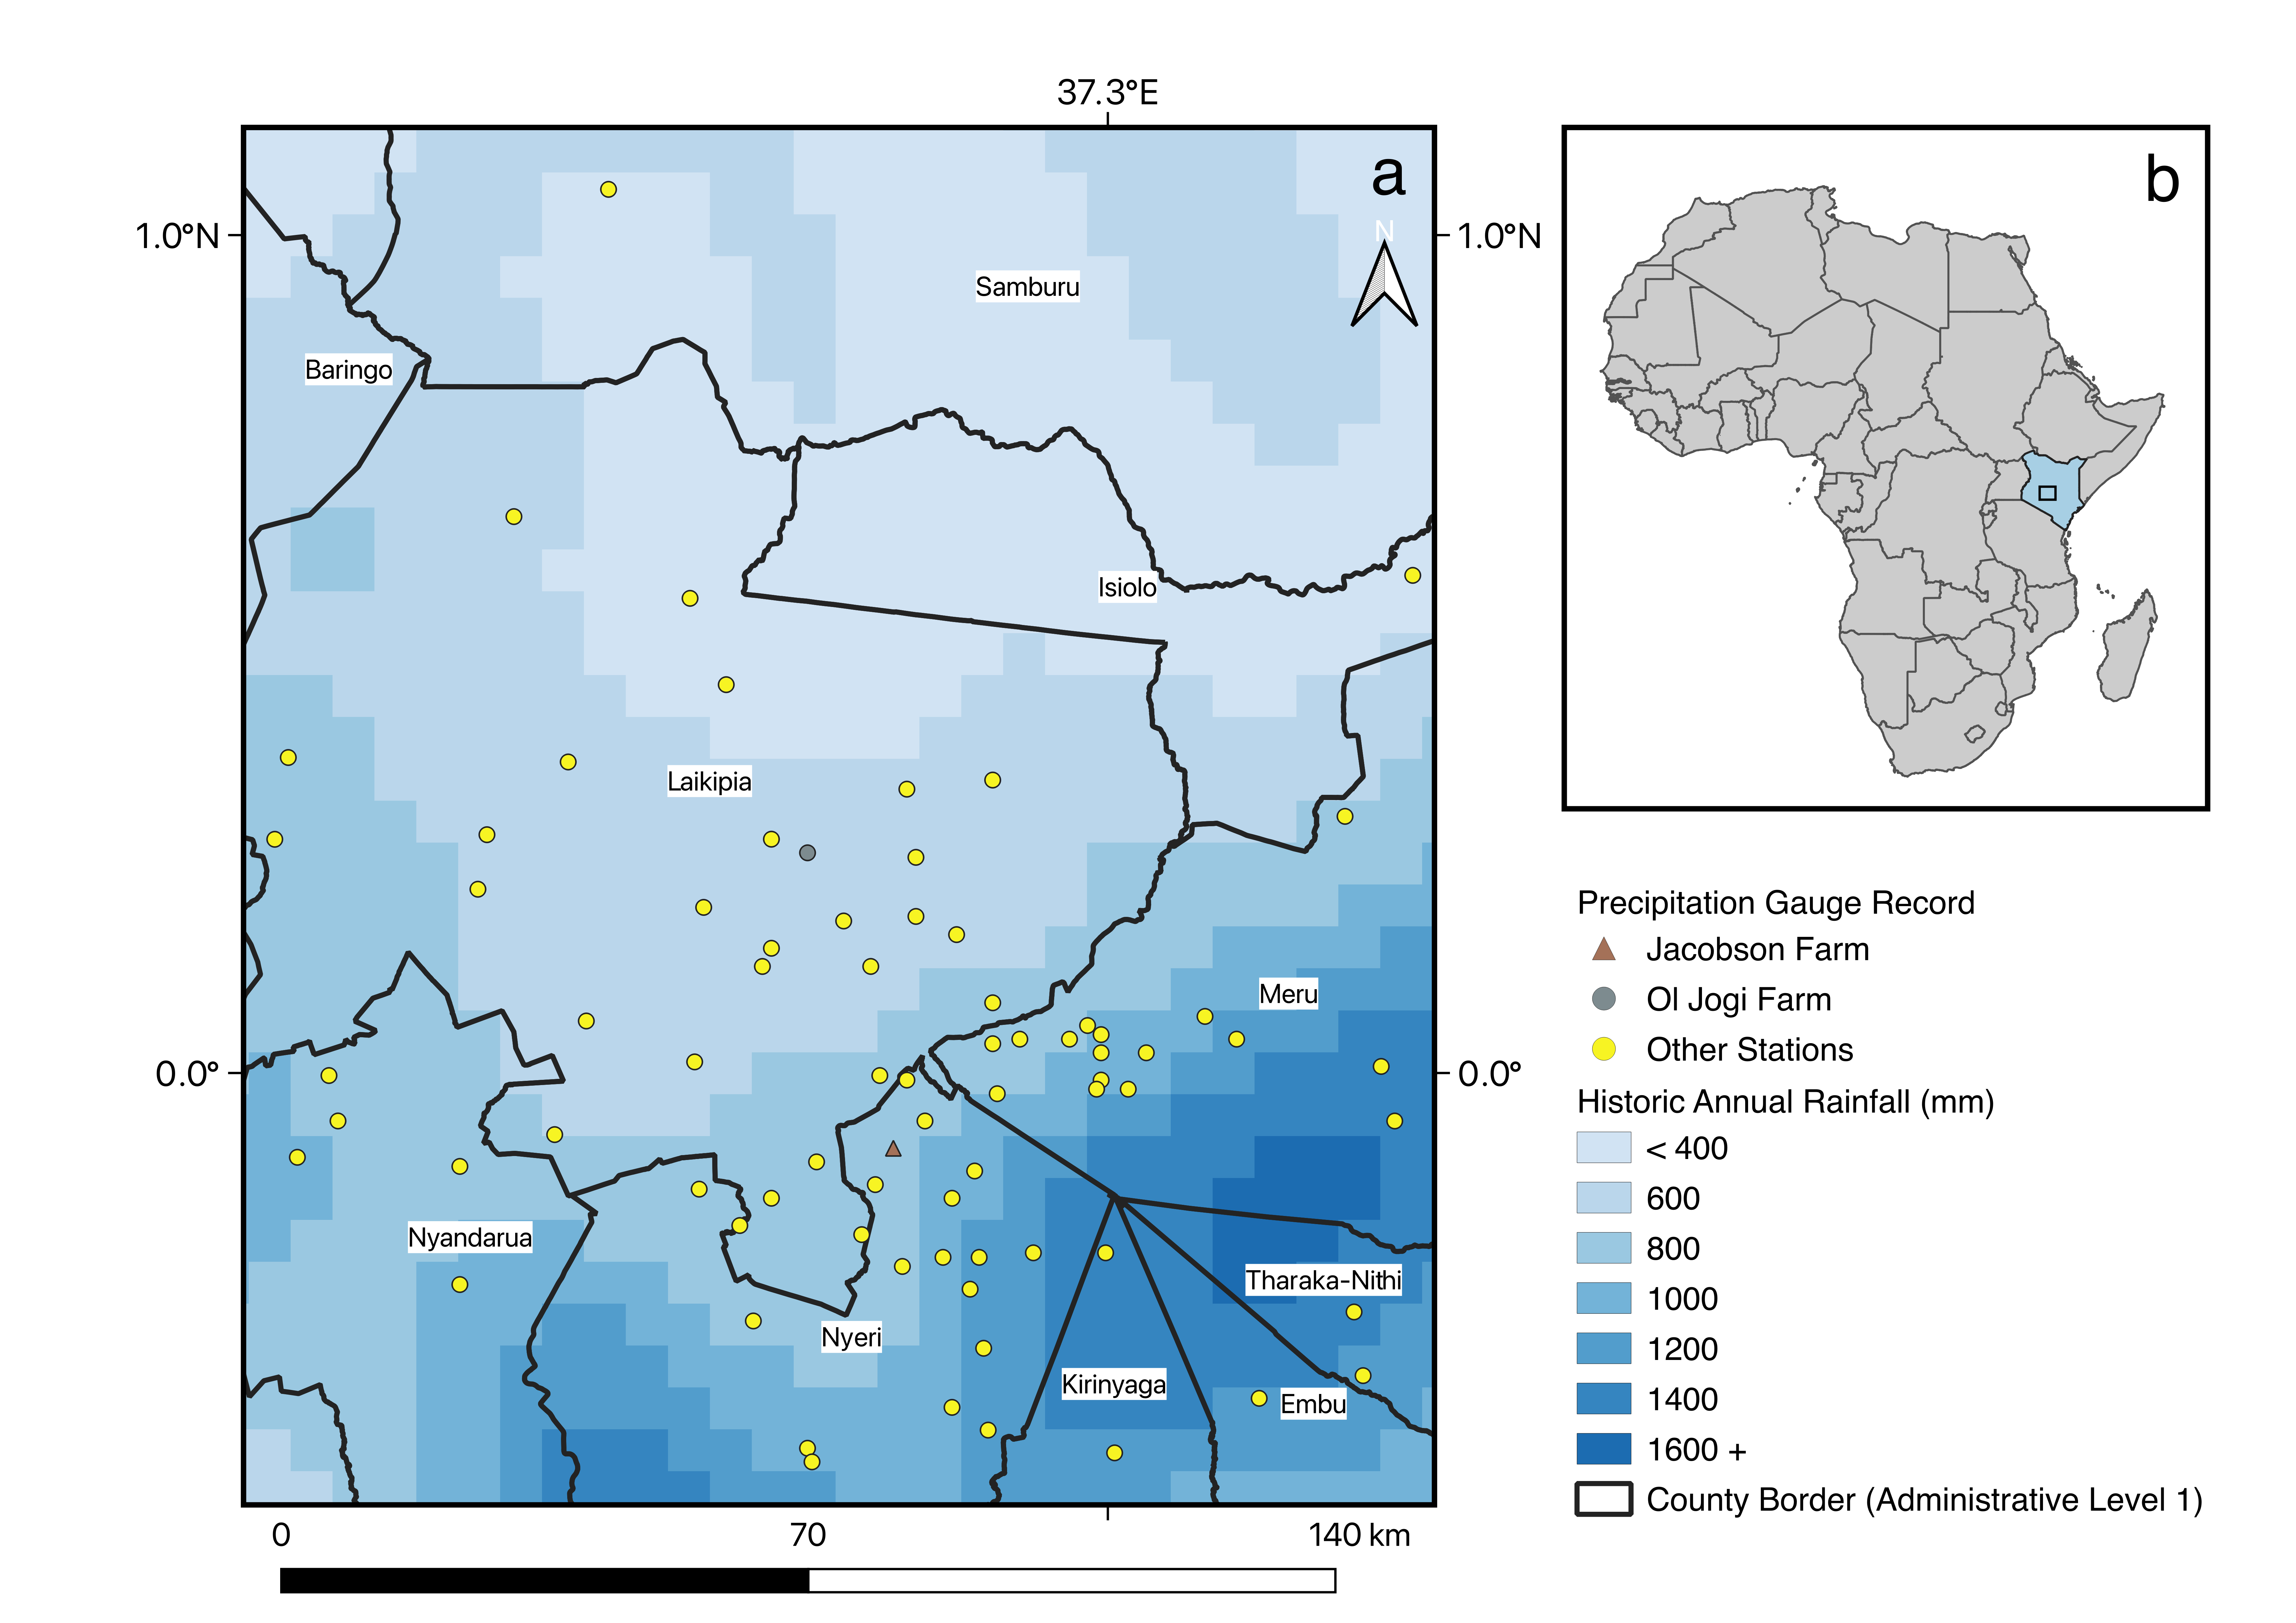
\includegraphics[width=100mm]{map.png}
\caption{Maps showing: a) Study site in Kenya noted by black box; b) Inset of map within Kenya. Point data is from 80 stations. Jacobson Farm and Ol Jogi Farm are denoted with a triangle and circle icon, respectively. Shades of blue indicate historic annual rainfall based on enhanced CHIRPS data (a blend of 710 quality controlled station observations with CHIRPS data) averaged over January Dekad 1 to December Dekad 3 1983-2016. Contours were delineated using the GeoClim Contour Tool using an interval of 200 mm.}
\label{fig:map}
\end{figure}

%--------------------------------------------------------------------%
%                                                                    %
%  METHODS                                                           %
%                                                                    %
%--------------------------------------------------------------------%

\section{Methods}

% Methods section consists of:
% 2.1 Study Site [sections/study_site.tex]
%   2.1.1 Soils
%   2.1.2 Climate
%   2.1.3 Crops
% 2.2 Model Description [sections/model_description.tex]
%    2.2.1 Hydrological Water Balance
%    2.2.2 Plant Water Stress
%    2.2.3 Crop Yield
% 2.3 Model Implementation [sections/model_implementation.tex]
%
%--------------------------------------------------------------------%
%                                                                    %
%  STUDY SITE (sections/study_site.tex)                              %
%                                                                    %
%--------------------------------------------------------------------%
\subsection{Study Site}

We apply our model to the smallholder farming communities on the western slope of Mount Kenya, specifically the Laikipia plateau, in east Africa as shown in Figure \ref{fig:map}. Laikipia county is located on the western (leeward) side of Mount Kenya and is adjacent to Meru and Nyeri counties in central Kenya. The county comprises smallholder agriculturalists, growing urban areas, and wildlife conservatories that attract tourism. The presence of dryland agriculturalists along a heterogeneous rainfall gradient makes the area suitable for an analysis of rainfall variability and cropping outcomes. The main cropping season for maize is planting around day 100 (first week of April) and harvesting around day 300 (last week of October) \cite{Ray2015}. % The study site receives on average 600-900 mm of rain per year and generally experiences two growing seasons around April and October \citep{Schmocker2016}.

Laikipia is a semiarid region prone to severe water deficits due to unreliable rainfall and high spatial and temporal variability. Rainfall in Kenya is characterized by a high coefficient of variability, which is common to semiarid environments \cite{herrero2010climate}. Furthermore, Laikipia has a heterogeneous landscape and complex topography that results in a rainfall gradient from 800-900 mm at the foothills of Mount Kenya to less than 500 mm in the northern end of the county \cite{wiesmann1998sustainable}. The annual distribution of rainfall is bimodal with two rainy seasons: the long (roughly March through May) and short (roughly October through December) rains. 

The Laikipia region of Kenya serves as an ideal study site to model the relationships between smallholder agriculture and climate variability for two reasons: (1) the tight couplings between food production and rainfall and (2) the prevalence of maize cultivation under various rainfall climatologies. In the region's drylands smallholder farmers face considerable challenges as rainfall arrives in pulses and in limited quantities for the majority of the year. Because the country has experienced a number of droughts in recent years, the Government of Kenya is especially interested in drought mitigation and increasing food security \cite{Kenya2010-jf}. Maize is an appropriate crop to study because it is grown under rainfed conditions and is an annual crop subject to both intermittent and terminal drought. Intermittent drought is caused by finite periods of inadequate water availability which does not necessarily result in crop failure whereas terminal drought is a progressive reduction in water availability that leads to crop failure before the end of the growing season \cite{neumann2008coping}.

\subsubsection{Soil Types}
We use the ISRIC Africa SoilGrids soil data base \cite{isric} to determine the soil textures found at depth 5-15 cm in our study site (Figure \ref{fig:map}). The region has a heterogeneous mix of soil textures. The most prevalent soil textures, at the points of the rainfall gauges, are clay, clay loam and sandy clay loam. Soils in our catchment are geologically young soils derived from basaltic volcanic rock and are generally fertile but susceptible to erosion. The clay soils have high water storage capacities, which can be suitable for growing maize \cite{muchena1988soils}. In Table \ref{soil} we show the corresponding values for the soil matrix potential at the hygroscopic point $\Psi_{s_{h}}$, and at field capacity $\Psi_{s_{fc}}$, the porosity $n$, and the saturated hydraulic conductivity $K_s$ according to the values found in \citeA{clapp1978empirical}.

\subsubsection{Historical Trends in Rainfall} \label{historic-rainfall}

We use long-term records of daily rainfall data for stations across the study site provided by the Centre for Training and Integrated Research in Arid and Semi-Arid Lands Development (CETRAD) in Nanyuki, Kenya. The gauges, shown in Figure \ref{fig:map}, have record lengths between 7 to 79 years. For computing statistics in Table \ref{table:mk}, we used stations with records of 40+ years. We considered temporal trends in the two parameters: $\alpha$, the average depth per rain event and $\lambda$, the average storm frequency per day during the two rainy seasons: long (March-May) and short (October-December) rains. To analyze inter-annual trends in the total seasonal rainfall and alpha and lambda parameters for the two seasons, we used a modified Mann-Kendall statistical test and the Theil-Sen estimator. Because the daily rainfall data is serially correlated, we use a variance corrected Mann-Kendall test proposed by \citeA{yue2004mann}, which detrends the serially correlated data and calculates an effective sample size using the lag-1 autocorrelation coefficient. We used the modified-mk package in R \cite{mmk}. 

\begin{figure}%[ht]
\centering
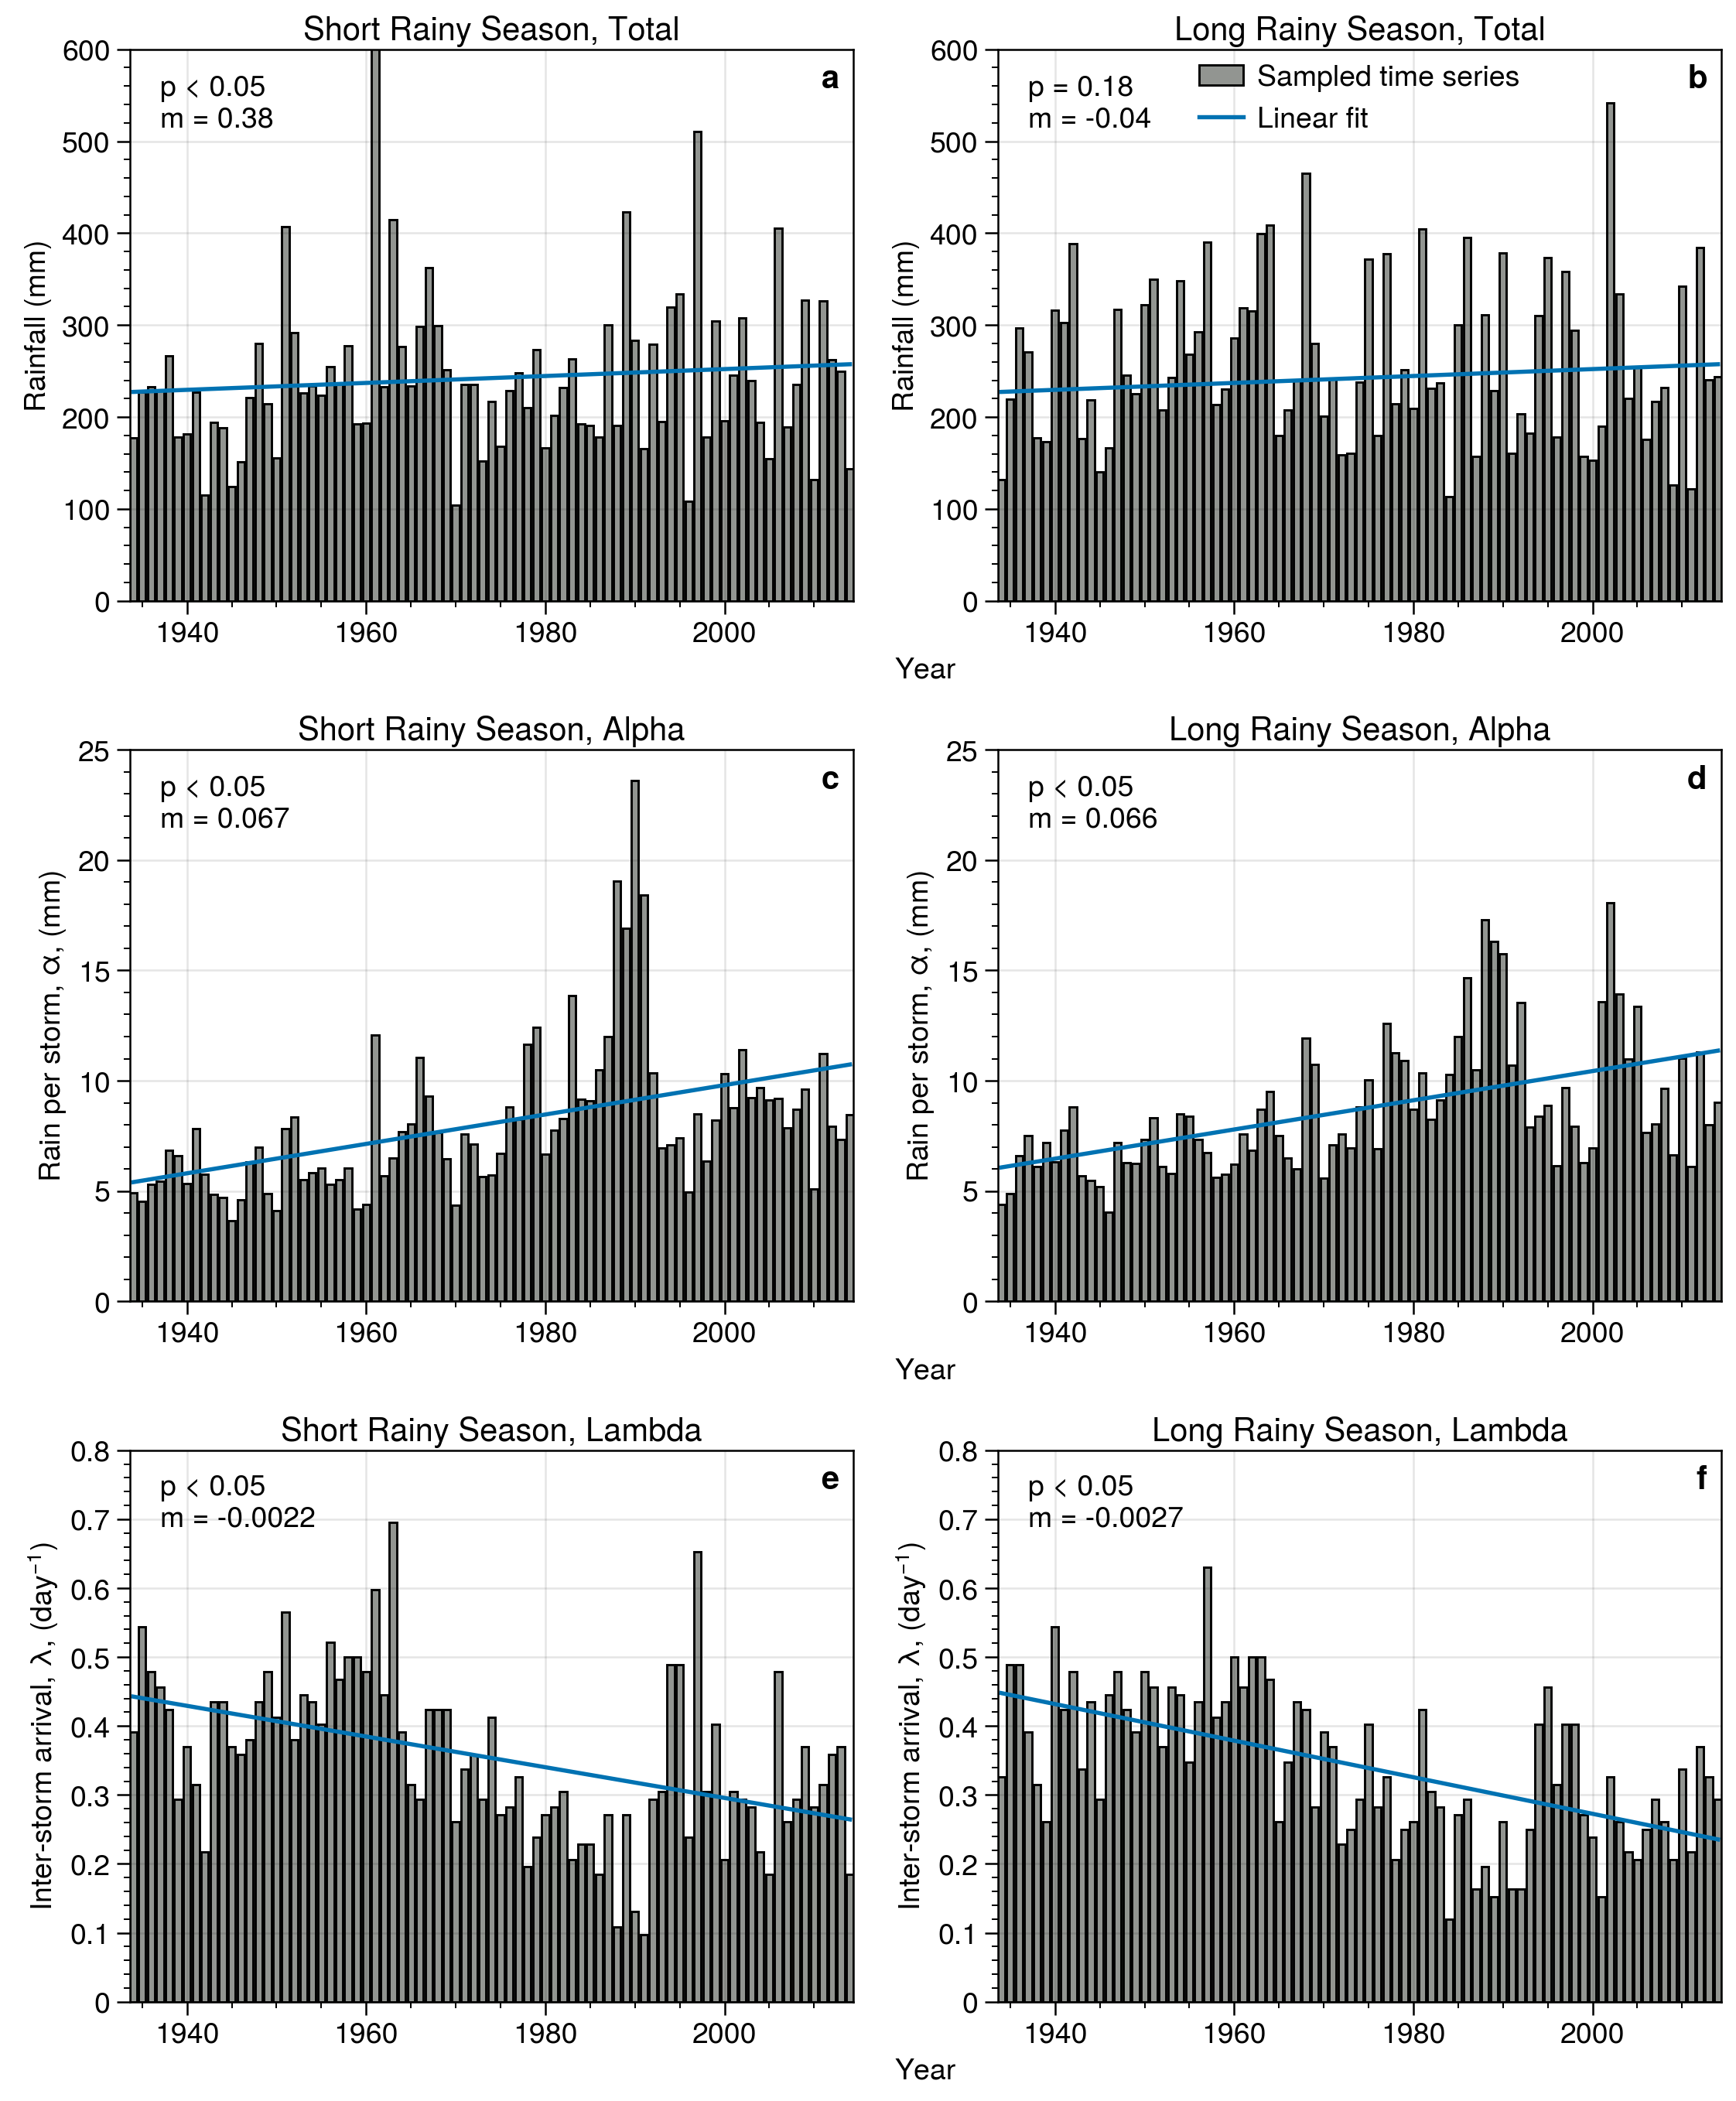
\includegraphics[width=155mm]{jacobson_ts.png}
\caption{Time series for the Jacobson Farm station which has a 79-year record length. Significant trends (p $<$0.05) are shown in plots a, c, d, e, f per the modified Mann-Kendall test.}
\label{fig:jacobson}
\end{figure}

\subsubsection{Maize Varieties and Yields}

In addition to being a function of environmental conditions and management decisions, total yields also depend on the maize variety. To define maximum potential yields for our simulations, we use empirical yield potentials for maize varieties typically grown by smallholder farmers in Laikipia. These data were sourced from Kenya Seed Company (see Figure \ref{fig:ksc}). We use the linear regression trend to set maximum potential yields for a range of maize varieties with maturity periods between 80 and 185 days. For each maize variety, we calculate a maximum potential yield, $Y_{max}$, which is used in Eq.~\ref{eq:yield}.

%Not actually including the text below, but could if we want to reduce max. yields again.
%Because potential yields are location-specific and the result of seed trials where water and nutrients are not limiting factors and biotic stress is controlled \cite{evans1993processes}, we altered the maximum yields to be more realistic with realized yields in Kenyan agriculture. Mention that this is different from actual yield (ya). We determined that a reasonable range of maize yields, irrespective of variety, is between 0.92 and 2.22 t/ha \cite{davenport2019using}. Therefore, we altered the minimum (1.28 t/ha) and maximum (5.04 t/ha) yield potentials from the seed companies based on the range in \cite{davenport2019using}, which led to a reduction of maximum values by 44\%. 

\begin{figure}%[ht]
\centering
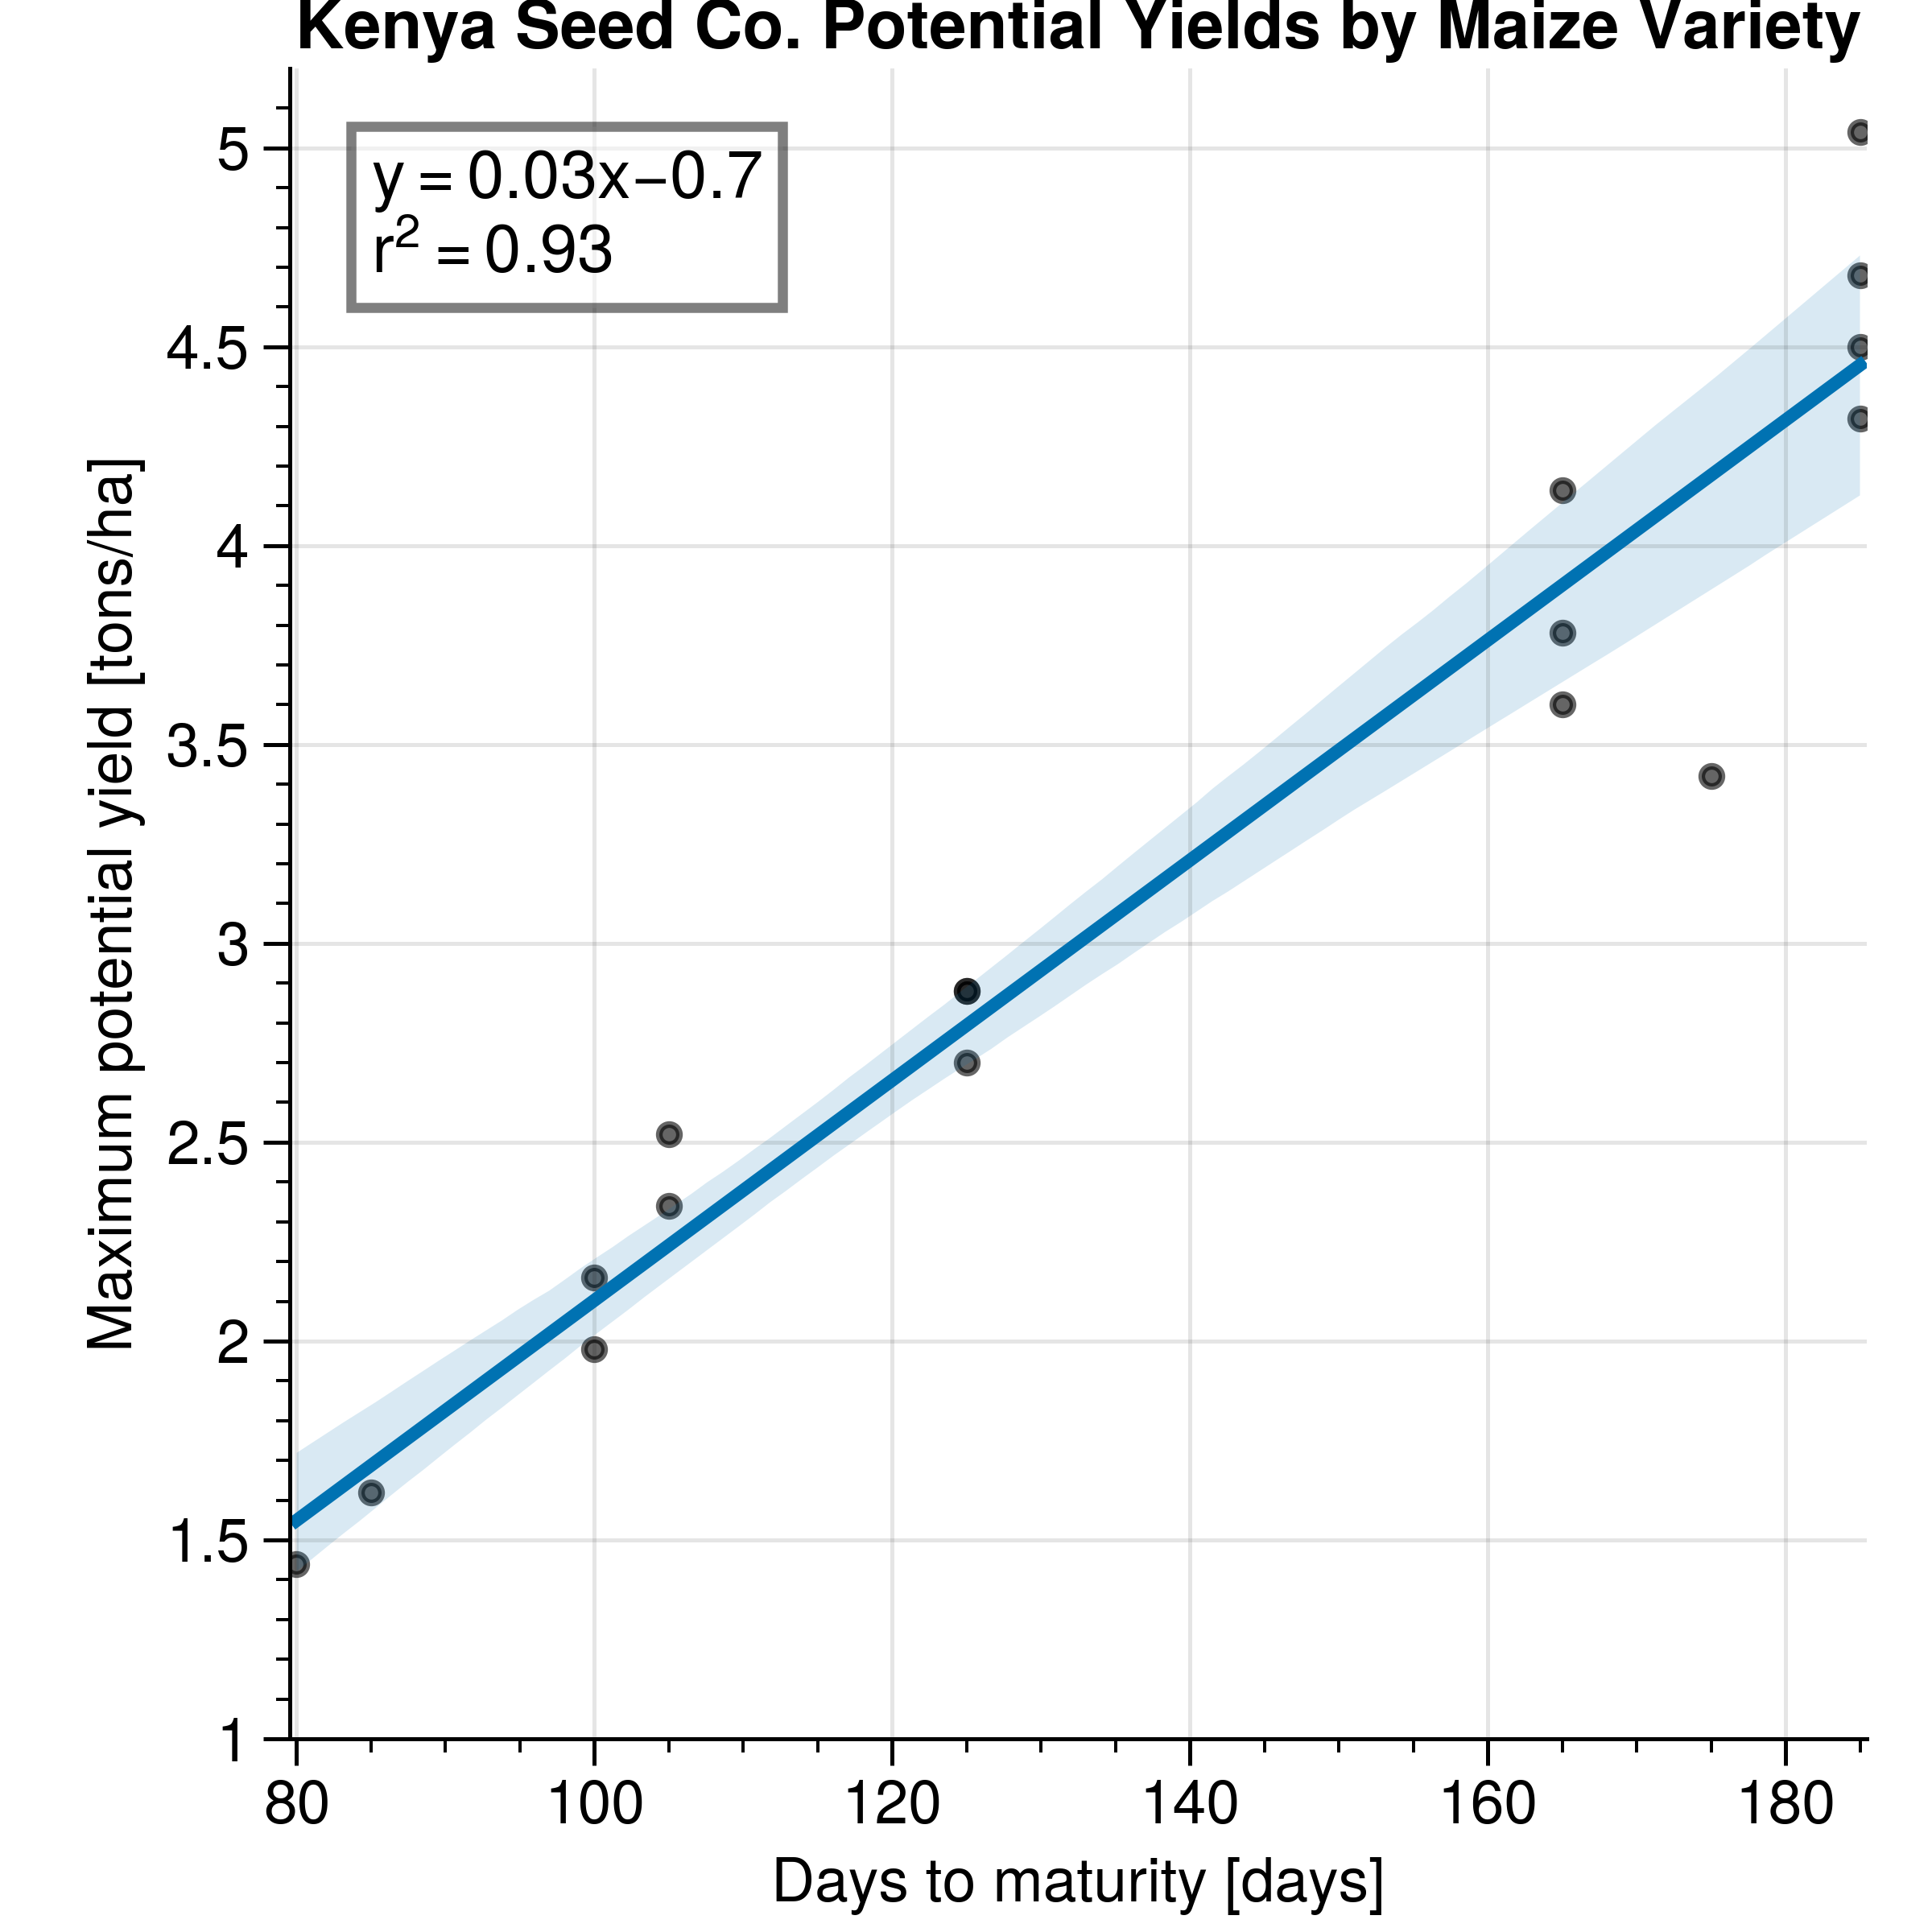
\includegraphics[width=80mm]{fig3_ksc.png}
\caption{Linear regression with 95\% confidence interval. Data are maize varieties sold by Kenya Seed Company. We removed two varieties from the dataset (PH1 and PH4) because the days to maturity information from Kenya Seed contradicted what is known about these four-month varieties. Data retrieved August 19 2019, from https://web.archive.org/web/20190216031348/http://kenyaseed.com/gallery/maize/.}

% Pretty sure that WRR is okay with having the citation in text as opposed to the reference list. If I do need it in the biblio use something like this: Highland maize varieties. (2019, February 16.) Kenya Seed Company Ltd. Retrieved August 19, 2019, from https://web.archive.org/web/20190216031348/http://kenyaseed.com/gallery/maize/. 

\label{fig:ksc}
\end{figure}

\begin{table}
\caption{Parameters associated with three prominent soil textures found within the study site.}
\centering
\begin{tabular}{l cccccc}
\hline
 Soil type  &  $\Psi_{s}$ (MPa)$^{b}$ & $b$$^{b}$ & $K_s$ (cm/d)$^{b}$ & $n$$^{b}$ & $s_h$ & $s_{fc}$ \\
\hline
  Clay & $-3.97 \times 10^{-3} $ &  11.4 & 11.1 & 0.482 & 0.503 & 0.830
  \\
  Clay loam  & $-6.17 \times 10^{-3}$  & 8.52 & 21.2 & 0.476 & 0.420 & 0.821 
  \\
  Sandy clay loam & $-2.93 \times 10^{-3}$ &  7.12 & 54.4 & 0.420 & 0.319 & 0.711
  \\
\hline
\multicolumn{7}{l}{$^{a}$We calculated values of $s_h$ and $s_{fc}$ assuming a soil water potential $\Psi_{h}=-10.0$ MPa} \\
\multicolumn{7}{l}{and $\Psi_{sfc} = -0.03$ MPa \cite{Laio2001-fe}.} \\
\multicolumn{7}{l}{$^{b}$\citeA{clapp1978empirical}.} \\
\end{tabular}
\label{soil}
\end{table}

%% SIDEWAYS FIGURE and TABLE
% AGU prefers the use of {sidewaystable} over {landscapetable} as it causes fewer problems.
%
 \begin{sidewaystable}
 \caption{Characteristics of rain gauges used in model simulations.$^{a}$}
\label{locations}
 \begin{tabular}{lcccccc}
\hline
Site &  Latitude &  Longitude &  Mean Annual Rainfall, mm & Altitude, m.a.s.l. & Start Year & End Year\\
\hline
Jacobson Farm & 0.04 & 37.04 & 735 & 1875 & 1934 & 2014 \\ %   0.040436,  37.043195
Ol Jogi Farm & 0.31 &  36.94 & 538 & 1741 & 1967 & 1999 \\ % Full lat, long 0.312581, 36.942360
\hline
\multicolumn{7}{l}{$^{a}$Start and end years are the years when the rainfall records began and ended for each rain gauge.}
 \end{tabular}
 \end{sidewaystable}

% \begin{table}
% \caption{Characteristics of rain gauges used in model simulations.}
% \begin{tabular}{lcccc}
% \hline
% Site &  Latitude &  Longitude &  Mean Annual Rainfall, mm & Altitude, m.a.s.l. \\
% \hline
% Jacobson Farm & 0.04 & 37.04 & 735 & 1875  \\ %   0.040436,  37.043195
% Ol Jogi Farm & 0.31 &  36.94 & 538 & 1741  \\ % Full lat, long 0.312581, 36.942360
% \hline
% \end{tabular}
% \label{locations}
% \end{table}
% % Could also put Record (years)

%--------------------------------------------------------------------%
%                                                                    %
%  MODEL DESCRIPTION (sections/model_description.tex)                %
%                                                                    %
%--------------------------------------------------------------------%
\subsection{Model Description}
\subsubsection{Hydrological Water Balance}
To characterize the field-scale water balance we use a simple single-layer model of soil moisture at a point. The overall water balance is given by:

\begin{equation}
\label{eq:h2o}
    n Z_r \frac{\text{d}s(t)}{\text{d}t} = R(t) - ET(s(t)) - L(s(t)) - Q(s(t)),
\end{equation}

\noindent
where $n$ is porosity [-], $Z_{\text{r}}$ is the rooting depth [mm], $s(t)$ is the saturation, or relative soil moisture content ($0 \leq s(t) \leq 1$), $R(t)$ is the rainfall rate [mm day$^{-1}$], $E(s(t))$ is the rate of evapotranspiration [mm day$^{-1}$], $L(s(t))$ is the rate of leakage [mm day$^{-1}$], and $Q(s(t),t)$ is the runoff rate [mm day$^{-1}$]. This is analogous to Eq. 1 from Rodriguez-Iturbe, et al. (2001), with the rate of interception by the canopy taken to be 0. 

In maize systems, rainfall interception by the canopy will be highest during tasseling (reproductive) and maturity stages \cite{zheng2018rainfall}. The degree to which rainfall is intercepted depends on a number of factors that can be site and canopy-specific. For instance, recent field studies in China, Iran and Indonesia indicate that canopy partitioning varies greatly and results are site-specific \cite{van2001modelling, zheng2018rainfall, nazari2020rainfall}. Because there are no field studies of rainfall interception by maize in Kenya (only studies that investigate the role of intercropping \textit{Grevillea robusta} with maize, e.g. \citeA{ong2000productivity, jackson2000measured}), we chose not to include interception in the model.

\paragraph{Rainfall}

Rainfall is treated as a non-stationary marked Poisson process. In each dekad (10-day increment) $i$, rainfall occurs with a probability, $\lambda_i$ [day$^{-1}$], and the depth of rainfall events are drawn from an exponential distribution with a mean value, $\alpha_i$ [mm]. Average dekadal values of $\lambda$ and $\alpha$ are estimated from a long-term rainfall record of daily station rainfall data, which was described previously in section \ref{historic-rainfall}. Using a fixed average $\lambda_i$ value for each dekad underestimates the variance in seasonal rainfall and does not accurately represent the observed coefficient of variation in seasonal rainfall for this region. Therefore, we allow dekadal $\lambda_i$ values to vary for each season by scaling all $\lambda_i$ values by a random, season-specific scale factor drawn from a normal distribution with a mean of 1 and a standard deviation of 0.35. This allows us to capture the coefficient of variation of seasonal rainfall at the Ol Jogi and Jacobson Farm stations. 

% Previously in this section but removed:
 %. with the probability density function

% \begin{equation}
% \label{eq:alpha}
%     f_{X,i}(x) = \frac{1}{\alpha_i} \mathrm{e}^{-\frac{x}{\alpha_i}}.
% \end{equation}

% This is repetitive I think
% We fit daily rainfall volumes from a long-term rainfall data set with 30+ years of data to an exponential distribution and return a fitted PDF for a given rainfall climatology (i.e. rain gauge). We test the fit of our exponential distribution with an empirical histogram to check that the modeled rainfall has a r-squared value above 0.9. To simulate daily rainfall values, we generate a time series of rainfall based on the parameters $\lambda$ and $\alpha$. To calculate an alpha value per month we find all of the daily rainfall values where rain was greater than 0 and fit the daily rainfall amounts to an exponential distribution to get a monthly alpha value. Then we calculate the monthly lambda value by dividing the number of rainy days by the total number of days in a month. Then to simulate daily rainfall values, we generate a time series of rainfall based on the parameters alpha and lambda and or the length of season. 

\paragraph{Evapotranspiration}

Evapotranspiration depends on both the soil moisture, $s$, and the time into the growing season, $t$. We separate evapotranspiration into its two components, soil evaporation $E(s,t)$ and plant transpiration $T(s,t)$ such that
\begin{equation}
\label{eq:ET1}
    ET(s,t) = E(s,t) + T(s,t).
\end{equation}

\noindent
Soil evaporation depends on both the amount of soil moisture and the extent of the crop canopy, which intercepts radiation and reduces energy available for soil evaporation. We define Evaporation as 

\begin{equation}
\label{eq:E}
    E(s,t) = \begin{cases}
        0   &   0 \leq s < s_{\text{h}}  \\
        \left( \frac{s-s_{\text{h}}}{1-s_{\text{h}}} \right) ^{q_{\text{e}}} ET_{\text{max}} \mathrm{e}^{-0.5 \cdot LAI(t)}  &   s_{\text{h}} \leq s \leq 1 \\
    \end{cases},
\end{equation}

\noindent
where $q_{\text{e}}$ represents the non-linear rate at which soil evaporation declines as soil moisture drops below saturation, $LAI$ denotes the crop leaf area index [mm$^2$ mm$^{-2}$], a measure of canopy density, and $s_{\text{h}}$ is the soil moisture at the hygroscopic point. $LAI(t)$ varies depending on the time into the growing season, $t$, and is calculated from the maximum leaf area index of a given crop, $LAI_{c,max}$ and the crop coefficient, $K_c(t)$, as follows:

\begin{equation}
\label{eq:lai}
    LAI(t) = LAI_{\text{c,\text{max}}} \frac{K_c(t)}{K_{c, \text{max}}}
\end{equation}

\noindent

\paragraph{Seasonal variation in the Crop coefficient}
The growing season is divided into four stages of crop phenology, through which the crop coefficient varies, peaking in mid-season after the reproductive stage. The crop coefficient is determined as

\begin{equation}
\label{eq:Kc}
    K_c(t) = \begin{cases}
        K_{c,\text{ini}}
            &   t \leq f_\text{i} \\[6pt]
            
        \frac{K_{c,\text{max}}-K_{c,\text{ini}}}{f_\text{d} - f_\text{i}} (t- f_\text{i}) + K_{c,\text{ini}}
            &   f_\text{i} < t \leq f_\text{d}   \\[6pt]
            
        K_{c,\text{max}}
            &   f_\text{d}  < t \leq f_\text{ms}   \\[6pt]
            
        \frac{K_{c, \text{eos}}-K_{c,\text{max}}} {f_\text{ls} - f_\text{ms}}  (t- f_\text{ms}) + K_{c,\text{max}}
            &   f_\text{ms} < t < f_\text{ls}  \\[6pt]

        K_{c,\text{eos}}
            &   t = f_\text{ls}
    \end{cases}
\end{equation}

\noindent
where $f_\text{i}$, $f_\text{d}$, $f_\text{ms}$, and $f_{\text{ls}}$ denote the time in days from the beginning of the growing season to the vegetative period (initial), reproductive period (development), maturity period (mid-season), and end of season (late season), respectively. The values of $K_c$ during vegetative and ripening periods are constant functions of time and the values of $K_c$ during reproductive and senescence stages are linearly interpolated between the values for the start and end of each period. We use crop coefficient ($K_c$) values based on those listed in FAO guidelines for 180-day maize (grain) in high altitude East Africa, which are defined as 0.3, 0.3, 1.2, 1.2, and 0.6 and correspond to 0\%, 16\%, 44\%, 76\% and 100\% of the growing season \cite{allen1998chapter}. We selected this metric for $K_c$ because it is widely used in the Crop Water Requirement Satisfaction Index (WRSI) \cite{senay2004crop} when locally appropriate values are absent. % the initial, mid-season, and end of season, respectively. 
%\citeA{allen1998chapter} provides crop development stages for a 180-day variety, which we use in our calculation of crop coefficient: $L_{\text{ini}=30}$, $L_{\text{dev}}$ = 50, $L_{\text{mid}}$ = 60, $L_{\text{late}}$ = 40. 

The rate of plant transpiration, $T(s)$, is given as

\begin{equation}
\label{eq:T}
    T(s) = \begin{cases}
        0   &   s < s_{\text{w}}  \\
        \frac{s - s_{\text{w}}}{s^* - s_{\text{w}}} K_c T_{\text{max}}    &   s_{\text{w}} \leq s < s^*  \\
        K_c T_{\text{max}}  &   s^* \leq s \leq 1 \\
    \end{cases}
\end{equation}

\noindent
where $T_{\text{max}}$ is the maximum transpiration rate of the plant, $s_{\text{w}}$ is the soil moisture at the wilting point, and, $s^{*}$ is the soil moisture at the stress point.

Having solved for the components of Eq.~\ref{eq:ET1}, we can use Eqs.~\ref{eq:E} and ~\ref{eq:T} express $ET(s)$ as follows:

\begin{equation}
\label{eq:ET2}
    ET(s) = \begin{cases}
    0   &   0 \leq s < s_{\text{h}}   \\[6pt]
    \left( \frac{s-s_{\text{h}}}{1-s_{\text{h}}} \right) ^{q_{\text{e}}} ET_{\text{max}} \mathrm{e}^{-0.5 \cdot LAI} 
        &   s_{\text{h}} \leq s < s_{\text{w}}   \\[6pt]

    \left( \frac{s-s_{\text{h}}}{1-s_{\text{h}}} \right) ^{q_{\text{e}}} ET_{\text{max}} \mathrm{e}^{-0.5 \cdot LAI} + \frac{s - s_{\text{w}}}{s^* - s_{\text{w}}} K_c T_{\text{max}} 
        &   s_{\text{w}} \leq s < s^*   \\[6pt]
    \left( \frac{s-s_{\text{h}}}{1-s_{\text{h}}} \right) ^{q_{\text{e}}} ET_{\text{max}} \mathrm{e}^{-0.5 \cdot LAI} + 
    K_c T_{\text{max}}
        &   s^* \leq s \leq 1  
    \end{cases}
\end{equation}

Figure \ref{fig:et} shows the functional form of evaporation and transpiration as a function of relative soil moisture content for a clay loam soil in which $s_{\text{h}}$ is 0.42, $s_{\text{w}}$ is 0.53, and $s^{*}$ is 0.78.

\begin{figure}%[ht]
\centering
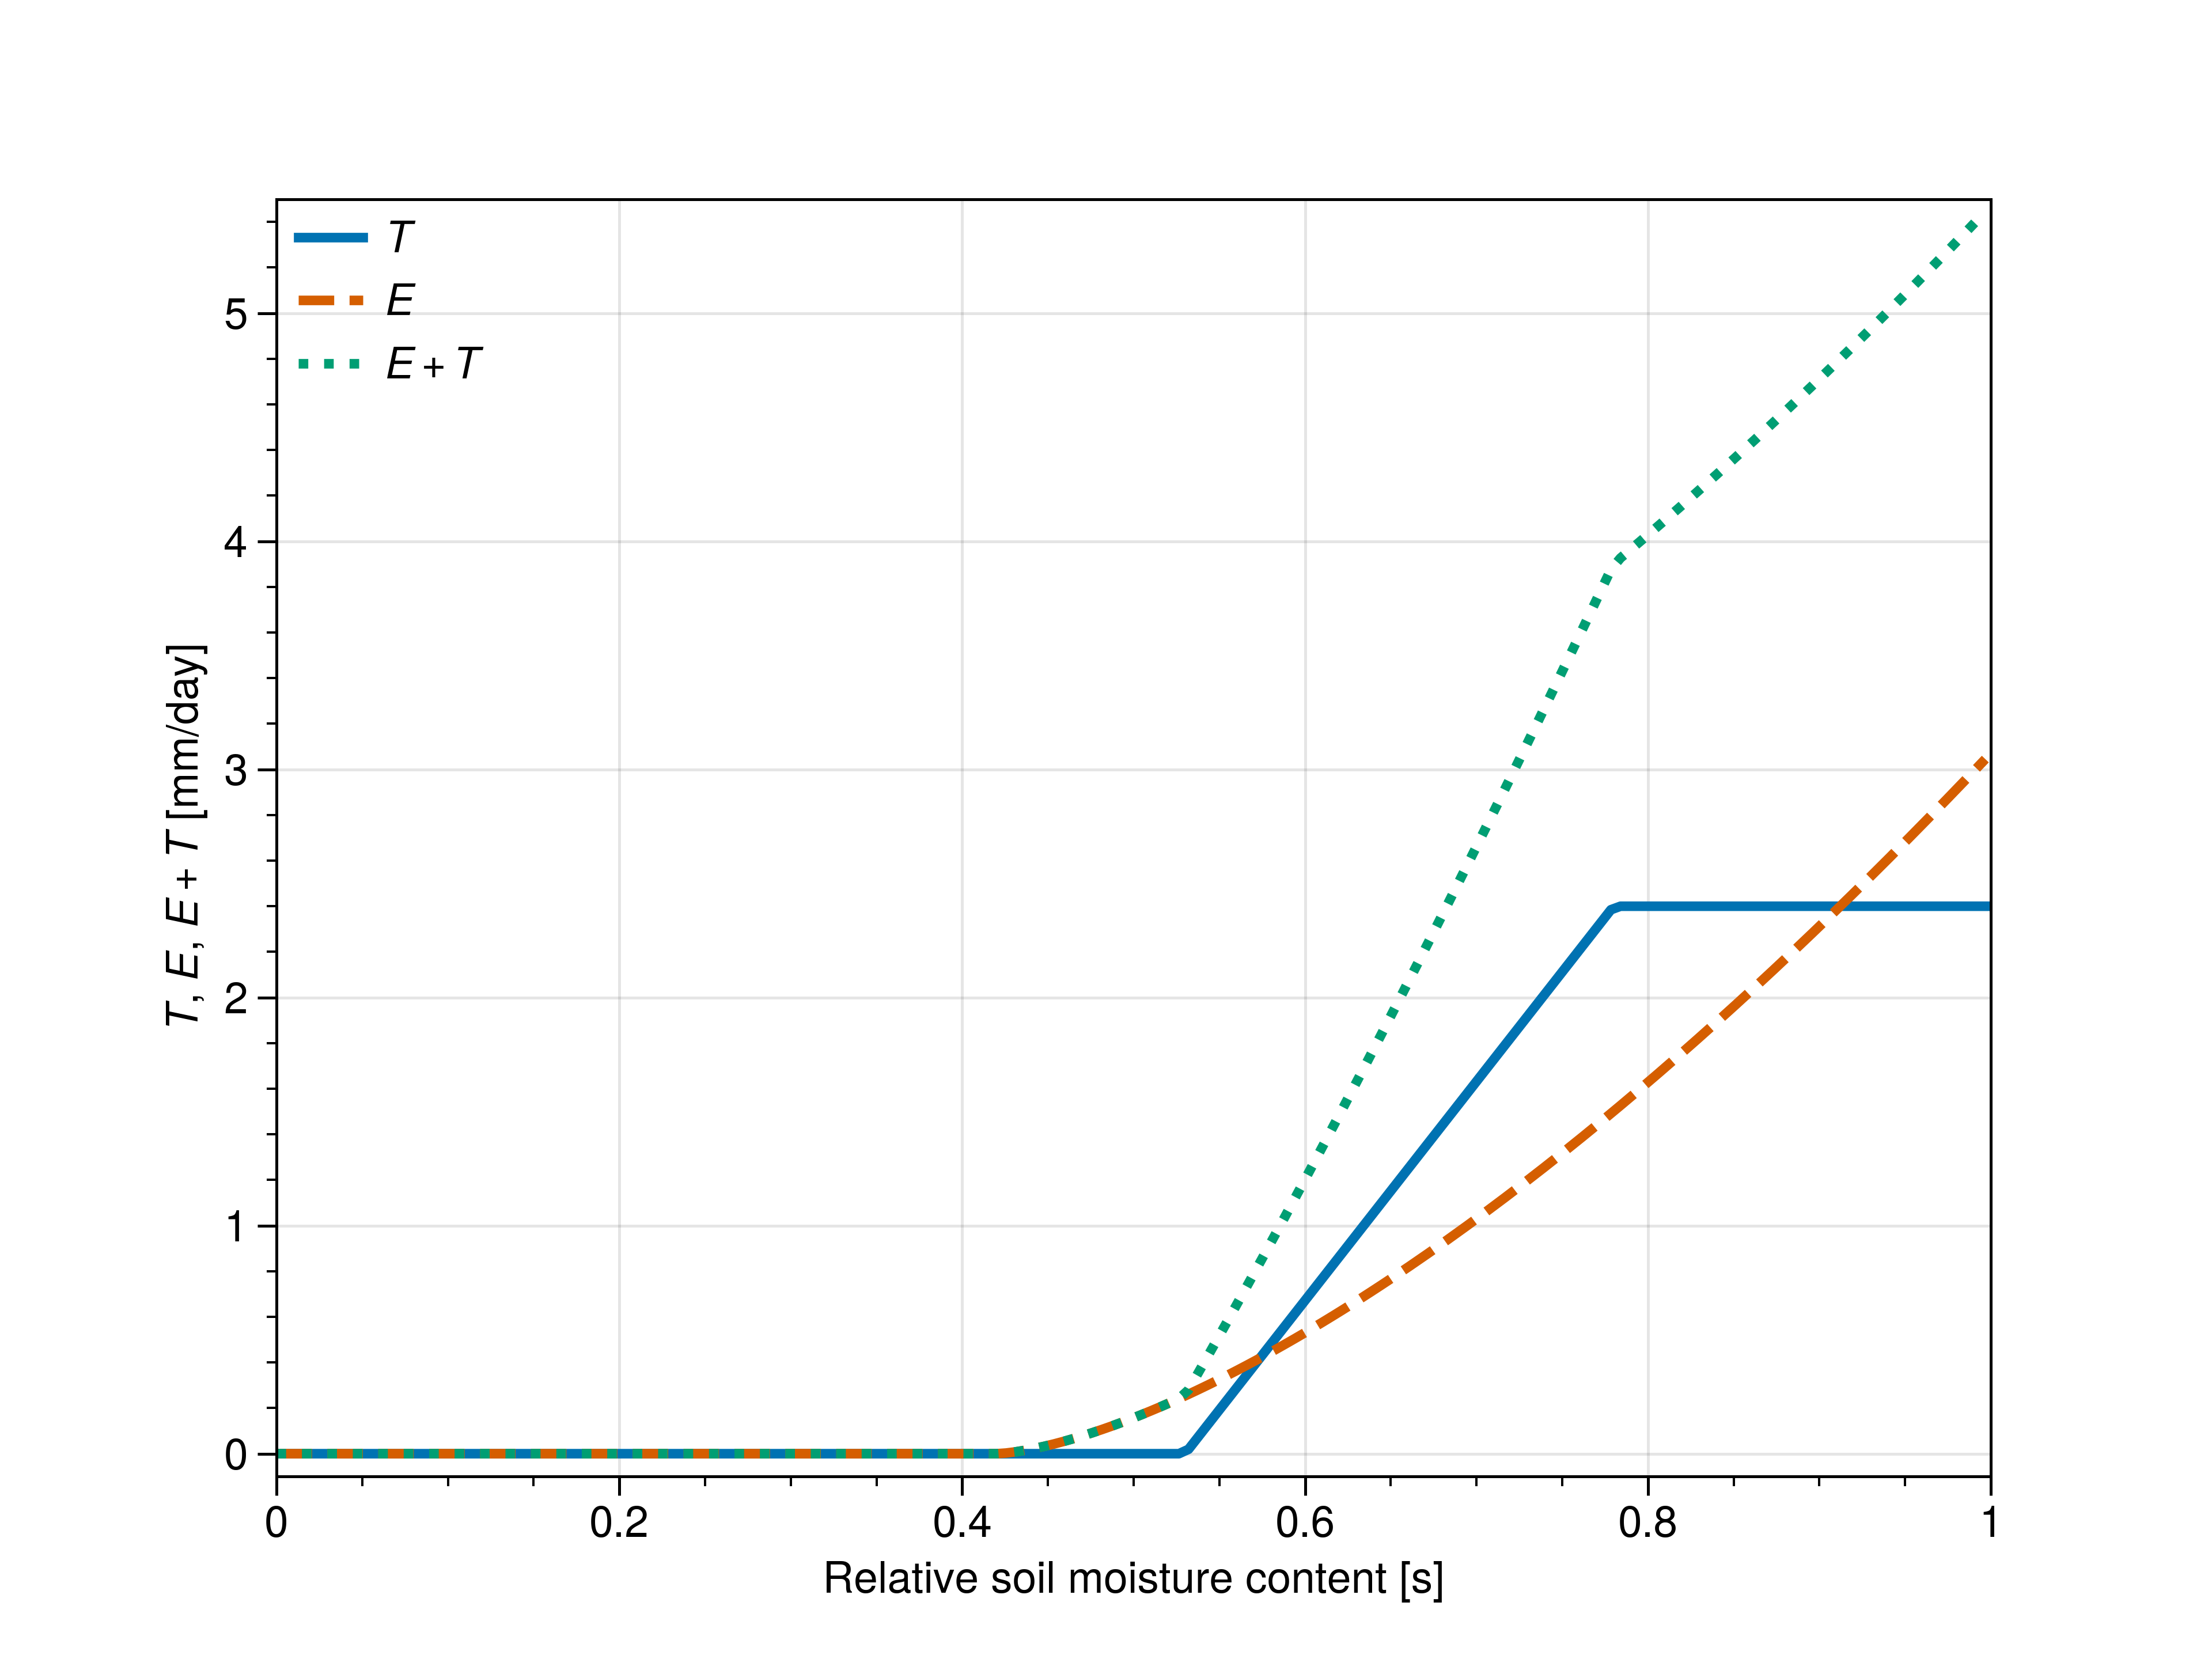
\includegraphics[width=100mm]{fig4_ET.png}
\caption{Evaporation, transpiration, and evapotranspiration as functions of relative soil moisture where LAI is 1.5 and $s_{\text{h}}$ is 0.42. Other climate and crop parameters are those listed in Table \ref{table:parameters}. }
\label{fig:et}
\end{figure}


\paragraph{Leakage}

Whenever daily soil moisture exceeds the soil field capacity, $s_{fc}$, we calculate leakage of water out of the plant root zone. The instantaneous rate of leakage is determined by the hydraulic conductivity, K(s) [mm/day], which is given by

\begin{equation}
\label{eq:K_s}
    L(s) = K(s) = \frac{K_s} {\mathrm{e}^{\beta(1-s_{\text{fc}})}-1} (\mathrm{e}^{\beta(s-s_{\text{fc}})}-1),
\end{equation}

\noindent
where $K_s$ is the saturated hydraulic conductivity [mm/day] and $\beta$ is a soil-specific parameter that governs the shape of the relationship between saturation and hydraulic conductivity; that is, $\beta = 2b + 4$, where $b$ is a  coefficient governing the power-law form of the soil-water retention curve \cite{Laio2001-fe}. 

\begin{equation}
    \varPsi_s = \overline{\varPsi}_s \, s^{-b}
\end{equation}

\noindent
where $\varPsi_s$ is the soil matrix potential at a given value of soil moisture and $\overline{\varPsi}_s$ is the geometric mean of the soil matrix potential values in the curve. Values of $b$ are based on soil texture and are taken from the empirically-determined coefficients presented in \citeA{clapp1978empirical}. 

Following an input of rainfall such that $s_0 >  s_{\text{fc}}$, Eq.~\ref{eq:h2o} becomes an expression of soil moisture decay. In the absence of evaporative losses, we can simplify leakage to

\begin{equation}
\label{eq:loss}
    L(s) = - n Z_{\text{r}} \frac{\text{d}s} {\text{d}t} 
\end{equation}

Then we use Eqs.~ \ref{eq:K_s} and \ref{eq:loss} to solve for the initial condition, $s_0$, which yields the solution for total daily leakage when $s >  s_{\text{fc}}$: 

\begin{equation}
\label{eq:L}
    L= \frac{n Z_{\text{r}}}{\beta} \ln{\left[ \mathrm{e}^{\beta (s_0 - s_{\text{fc}})} - \mathrm{e}^{-m \beta} (\mathrm{e}^{\beta (s_0 - s_{\text{fc}})} - 1 ) \right] }
\end{equation}

where 

\begin{equation}
\label{eq:m}
    m = \frac{K_s}{n Z_{\text{r}} \left( \mathrm{e}^{\beta (1 - s_{\text{fc}})} - 1 \right)}
\end{equation}


\paragraph{Runoff}

Our model only considers saturation excess overland flow, so that when the balance of daily rainfall, evaporation, and leakage leads to an excess of soil saturation, the excess is converted to surface runoff. Thus, we can write

\begin{equation}
\label{eq:Q}
    Q(s) = \begin{cases}
        0           &   0 \leq s \leq 1 \\
        (s-1) n Z_{\text{r}}  &   s > 1
    \end{cases}
\end{equation}


\vskip 24pt


\subsubsection{Plant Water Stress}

Water stress during the growing season affects the physiology of plants and is crucial in determining the success of a crop. Soil moisture excursions below the wilting point, $s_w$, and the point at which transpiration is reduced, $s^{*}$, can lead to reduced biomass production and eventual crop failure. By defining the duration and frequency of soil moisture deficits probabilistically, we gain insight into the yield reductions from intense water stress such as drought and the likelihood of crop failure. The mathematical derivations for these dynamics are described in previous work (e.g. \citeA{rodriguez2007ecohydrology}.)

First we calculate static water stress: a measure of the mean vegetation water stress stress incurred during a given excursion below $s^{*}$ \cite{Porporato2001-ui}.

\begin{equation}
\zeta(t) = \left[ \frac{s^*-s(t)}{s^*-s_w} \right]^{q_{\text{stress}}}\text{,        for } s_w \leq s(t) \leq s^*
\end{equation}

where $\zeta(t)$ is the static water stress and $q_{\text{stress}}$ represents the crop's sensitivity to the magnitude of excursions below the stress point.

Although the static stress describes the mean water deficit relative to $s^*$ and $s_w$, we are also interested in the duration and frequency of water deficit. Following the work of \citeA[p.~67]{rodriguez2007ecohydrology}, we also define two other random variables: the average length of time in days in which soil moisture is below the threshold, $T_\zeta$, and the number of times the threshold is crossed during a season, $n_\zeta$. Next, we calculate dynamic water stress, $\theta$, a measure of the crop's total water stress during the growing season that characterizes the duration and frequency of exposure to water stress:

\begin{equation}
    \theta = \begin{cases}
        \left( \frac{{\overline{\zeta} \, } \overline{{{T}}_{s*}}}{k{LGP}} \right)^{n^{-r}_{s^*}}
        &\text{,    }   \overline{\zeta} \, \overline{{T}_{s*}} < k{LGP} \\
        
        1  & \text{, }    {\overline{\zeta} \, } \overline{{{T}}_{s*}} \geq k{LGP}
    \end{cases}
\end{equation}

% \theta = \left( \frac{{\overline{\zeta} \, } \overline{{{T}}_{s*}}}{k{LGP}} \right)^{n^{-r}_{s^*}}\text{,        

% for }\overline{\zeta} \, \overline{{T}_{s*}} \leq k{LGP} %\leq s^*

where $\overline{\zeta}$ is the average static water stress incurred over the growing season; $\overline{T}_{s*}$ is the average duration of excursion; $n_s$ is the number of occurrences of these excursions during the growing season; $LGP$ is the length of the growing period in days; $k$ is the portion of the season that stress can occur before the crop fails; and $r$ is a normalization parameter for the number of excursion below the stress point. We use the values for $r$ and $k$ noted in Table \ref{table:parameters}. The $r$ parameter is defined  as in \citeA{Porporato2001-ui}, and the $k$ parameter is selected in order to approximate a characteristic rainfall yield relationship such as in \citeA{guan2017assessing}. Lastly, we calculate seasonal crop yields, $Y$, as a function of dynamic water stress:

\begin{equation}
\label{eq:yield}
Y = Y_{max}(1-\theta)
\end{equation}
where the maximum yield per unit area (hectare) is $Y_{max}$. % Not 100% sure here but I think the cite for this is Porporato et al. 2001.

% ~\ref{fig:vertprofile}

%--------------------------------------------------------------------%
%                                                                    %
%  MODEL IMPLEMENTATION (sections/model_implementation.tex)          %
%                                                                    %
%--------------------------------------------------------------------%
\subsection{Model Implementation}

%--------------------------------------------------------------------%
%                                                                    %
%  PARAMETER TABLE                                                   %
%                                                                    %
%--------------------------------------------------------------------%
\begin{table} %sideways
\caption{Model parameters and their sources.} %  References noted in footnote when needed. 
\label{table:parameters}
\centering
\begin{tabular}{lll l}
\hline
 Type & Parameter  & Value \\ % & Units 
\hline
 %Climate parameters &  $PET$ & 6 mm day$^{-1}$$^{a}$ \\ %& Potential Evapotranspiration 
  % Barron paper found daily potential ET between 3.7 and 5.5 mm Machakos Kenya (1200m asl), so 6 is a little high by okay.
   Climate parameters & $LGP$  & 180 days \\ %Length of season & \\ 
\hline
 Crop parameters &  $Z_{\text{r}}$  & 400 mm$^{a}$ \\ %& Rooting depth
 & $T_\text{max}$  & 4.0 mm day$^{-1}$   \\ %& Maximum crop water use
 & $ET_\text{max}$  & 6.5 mm day$^{-1}$$^{b}$ \\
 & $K_{c, \text{max}}$ &  1.2 (dim)$^{c}$ \\ %& Maximum crop coefficient
 & $LAI_\text{c}$  & 3.0 mm$^{2}$ mm$^{-2}$$^{d}$\\ %& Maximum Leaf Area Index
 & $q_\text{e}$ & 1.5 (dim) \\
 & $q_{\text{stress}}$ & 2 (dim) \\
 & $r$ & 0.5 (dim)$^{e}$ \\ % r = 0.5 in \cite{Porporato2001-ui} p. 739 (square root term)
 & $k$ & 0.2 (dim) \\ % k = 0.5 in \cite{Porporato2001-ui} p. 739
 & $Y_\text{max}$ & 3.2 t ha$^{-1}$ \\
 \hline
 Soil parameters (clay loam) & $s_w$ & 0.53 (dim)$^{f}$ \\ %& Wilting point in saturation
 & $s^*$ & 0.78 (dim)$^{f}$ \\ %& s star
 % See Table 3 for more params.
 \hline
 Simulation parameters & $N_{\text{sim}}$ & 10,000 seasons \\
 & $N_{\text{burn\_sim}}$  & 1,000 seasons \\ 
 & $T_\text{burn}$ & 60 days \\
 %% Extra variables, not including
 %  $n$   & 0.40 m$^{3}$ m$^{-3}$  & \citeA{williams2004soil}  \\ %& Porosity
 % $\rho$  & kg m$^{-3}$ & Density of water & 1000   \\
 % $g$  & m s$^{-2}$ & Acceleration of gravity & 9.8   \\
  %$K_s$ & cm min$^{-1}$ & Saturated hydraulic conductivity & 0.0417 &   %\citeA{clapp1978empirical} \\
  %$s$  &  & Relative soil moisture & [0,1]   \\
 % $s0$  &  & Initial soil moisture & 0.3   \\
 % $sw_\text{MPA}$  & -1.5 MPa   \\ %& Wilting point in water potential
  %$s^*_\text{MPA}$ & -0.05 MPa   \\ %& Water potential of maximum transpiration
  %$s_h$  & 0.04 &  Porporato et al. 2003?  \\ %& Soil hygroscopic point
  %$q$  &  & Exponent on the calc E curve & 1.5   \\
 % field\verb!_!capacity   & MPa & Field capacity & -33/1000 & \citeA{clapp1978empirical}  \\
  %$s_{fc}$ & 0.35 & Porporato et al. 2003?  \\ %& Field capacity
  %$Psi_{S_cm}$ & cm & Saturated water tension &  \\  
  %$Psi_{lcm}$ & cm & Leakage water tension &  \\  
  %$S$ & cm min$^{\frac{1}{2}}$ & Sorptivity &  \\
  %$\alpha$  & mm  & 10.0   \\ %& Average storm depth
  %$\lambda$  & day$^{-1}$  & 0.25\\ %& Storm frequency
  %$\xi$  & Plant water stress  & ...  \\
  %$\beta$ & 12.5 & \citeA{Laio2001-fe}   \\
\hline
\multicolumn{2}{l}{$^{a}$\citeA{nyakudya2014effect}} \\
\multicolumn{2}{l}{$^{b}$\citeA{barron2003dry}} \\
\multicolumn{2}{l}{$^{c}$\citeA{allen1998chapter}} \\
\multicolumn{2}{l}{$^{d}$\citeA{williams2004soil}} \\
\multicolumn{2}{l}{$^{e}$\citeA{Porporato2001-ui}} \\
\multicolumn{2}{l}{$^{f}$\citeA{clapp1978empirical}} \\
\end{tabular}
\end{table} %sideways

% this doesn't seem necessary
% \subsection{Probabilistic Description of Crop Development}
% In water-limited environments, plants operate at the interface between soil properties and climate dynamics \cite{Rodriguez-Iturbe2001-un}. Plants are impacted by the arid conditions they are in as well as actively use available water, which alters the soil-water balance. In turn, plants play an active role in impacting the hydroclimatic environment through soil-atmosphere interactions. Though large and complex processes govern the hydroclimatic dynamics in water-limited environments, we adhered to a simplified model of crop water use that has been demonstrated a viable method under similar dryland conditions \cite{Rodriguez-Iturbe2001-un, laio2001plants, Porporato2001-ui}. To preserve the essential features while simultaneously simplifying assumptions of temporal dynamics of soil moisture, we implemented a numerical modeling scheme to understand the role of different maize varietals on soil moisture in response to water stress. 

% The general form of the soil moisture balance follows... Co-author will add this section.

In order to conserve the water balance, we implement the model piecewise. First, we calculate saturation excess, $Q(t)$, which is caused by an input of rainfall that leads to the soil moisture being above saturation (i.e. $s>1$). Then we then calculate both leakage and evapotranspiration using the same $s$ value and within the same time step. Lastly, once we have values of $L(t)$ and $ET(t)$, we update the water balance and the soil moisture. 

We run the model for 10,000 simulations using the following initial conditions and parameters. We use the Ol Jogi Farm rainfall climatology (dekadal rainfall parameters estimated from daily rainfall records between 1967-1998), a clay loam soil texture, and 180-day maize variety, which are typical values for the study site. We selected a planting date of March 1 (Julian day 60) for model calibration and simulations. Farmers vary in their planting practice but generally plant at the start of the long rains after approximately 20 mm of rainfall has fallen. We selected March 1 because it was the most frequently planted week for the long rains among surveyed farmers in our study site. To determine the initial condition for our simulations, we first run the model for sixty days before the planting date and run 1,000 simulations to get an average value of $s$ for the first day of the season. Then we use this average value as the initial condition for each of our subsequent simulations of the growing season.

\subsubsection{Impacts of maize variety on farming outcomes}

To compare yield outcomes for different maize varieties, we run the simulations for three categories of varieties with different times to maturity that vary between 75 and 180 days: early maturing between 75 and 105 days, medium maturing between 110 and 140 days (inclusive), and late maturing between 145 to 180 days. Each category has 21 maize varieties, which are each simulated 500 times, resulting in 10,500 total simulations.

\subsubsection{Impacts of rainfall climatologies on farming outcomes}

We use two rainfall gauges to determine our $\alpha$ and $\lambda$ parameters, which are described in Table \ref{locations}. First, we use the long-term average Ol Jogi Farm rainfall climatology for running the model as this location is climatologically representative of semiarid small-scale producers in the region who depend on rainfall. We use this station for the model simulation results in sections \ref{non-stationarity} through \ref{cultivar_choice}.

We use the longest station gauge record (79 years), Jacobson Farm rainfall climatology, to analyze temporal changes in crop production and crop failure. We define three eras of crop production: two extreme conditions (1930s rainfall climatology and 2010s rainfall climatology) and the average rainfall conditions. We extract dekadal $\alpha$ and $\lambda$ values as follows. To represent average annual change in either parameter, we use the average dekadal $\alpha$ and $\lambda$ values, which considers the entire rainfall record and corresponds to the climate in the middle of the record. We adjust the long-term average values for each dekad in order to obtain historical (1930s) or present (2010s) values of the parameters in each dekad. To estimate the past, ``1930s", dekadal $\alpha$ and $\lambda$ values we simply apply the trend line to each of the individual average dekads. For example, we calculate the dekadal $\alpha$ for the 1930s climatology by taking the average dekadal alpha and subtracting it by the slope of the trend line multiplied by 40 years. For the present ``2010s" values we add the slope of the trend line multiplied by 40 years.  We then use these three sets of $\alpha$ and $\lambda$ values to run the simulations for the three subsetted periods. We run 100,000 simulations for each period. 

%%%%%%%%%%%%%%%%%%%%%%%%%%%%%%%%%%%%%%%%%%%%%%%%%%%%%%%%%%%%%%%%
\begin{table}
\caption{Summary of rainfall statistics with gauge record lengths greater than 40 years (n = 39) for short rains (SR, March through May), long rains (LR, October through December) or both seasons. We computed a modified Mann-Kendall test to designate significant trends (p $<$ 0.05). Data source: CETRAD.}
% Our results are consistent with \citeA{franz2010ecohydrological}): Total rainfall remains constant and increasing alpha and decreasing lambda trends for both seasons.
\centering
\begin{tabular}{llll l}
\\\hline
Parameter  & Season & Percent of stations  & Mean slope   & Standard  \\
description  & & with significant   & of all stations & error of \\ 
& & trends (p $<$ 0.05) & (Sen's method) & slopes \\
\hline
  Total rainfall [mm] & SR & 8.75 & 0.2863 & 0.4469 \\
   Total rainfall [mm] & LR & 1.25 & -1.115 & 0.5240 \\
   Annual rainfall [mm] & Both & 12.82 & -0.0673 & 0.6194 \\
   Average rain per storm  $\alpha$ [mm] & SR & 20.00 & 0.0654 & 0.0153 \\
  Average rain per storm  $\alpha$ [mm] & LR & 21.25 & 0.0641 & 0.0180 \\
   Average arrival rate of rain  $\lambda$ [day$^{-1}$]  & SR & 33.75 & -0.0010 & 0.0006 \\
   Average arrival rate of rain $\lambda$ [day$^{-1}$]  & LR & 32.50 & -0.0030 & 0.0005 
\\\hline
%\multicolumn{2}{l}{$^{a}$Footnote text here.}
\end{tabular}
\label{table:mk}
\end{table}


%--------------------------------------------------------------------%
%                                                                    %
%  RESULTS                                                           %
%                                                                    %
%--------------------------------------------------------------------%
\section{Results}
\subsection{Rainfall climatology trends}

We investigated inter-annual trends in seasonal totals, storm depth and inter-storm arrival rate for the two rainy seasons. Overall, we find that changes in seasonal totals are minimal across the stations, shown in Table \ref{table:mk}, and as visualized for Jacobson Farm in Figure \ref{fig:jacobson}. However, we do find significant trends for increasing intensity, $\alpha$, and decreasing frequency, $\lambda$ in both rainfall seasons ($p < 0.05$, Table \ref{table:mk}) using the modified Mann-Kendall statistical test. Comparatively, total rainfall for both seasons and annual rainfall shows a muted change with fewer stations showing significant trends. Our results are consistent with those of \citeA{franz2010ecohydrological}, which analyzed a less recent dataset of 11 stations in the same region. In Figure \ref{fig:jacobson}, we use the Jacobson Farm rain gauge which has the longest record (79  years) to show the shifts in rainfall processes that occur in this region. Here, we see that while total rainfall for either season does not change significantly, we see an increase in $\alpha$ and decrease in $\lambda$ over the period ($p < 0.05$, Fig. \ref{fig:jacobson}). This indicates that storms are becoming more intense and less frequent. The relevance of this inter-annual variability in rainfall is further discussed in section \ref{discussion}.

\subsection{Non-stationarity impacts of seasonal water availability} \label{non-stationarity}

Figure \ref{fig:threefigs_dekadal} (bottom panel) shows the average soil moisture content for 10,000 growing seasons of a 180 day variety planted in dekad 7 (approx. March 1) using the Ol Jogi rainfall climatology. The $\alpha$ and $\lambda$ parameters used to generate rainfall are variable over the 6 month period. The inter-storm arrival rate, $\lambda$, increases more than three-fold during the first 80 days (8 dekads) of the season while the average depth per storm, $\alpha$, exhibits stationary variation between 8-13 mm of rain (Fig. \ref{fig:threefigs_dekadal}, top). On dekad 15, the $\lambda$, drops and levels off indicating the cessation of the long rains season and the  $\alpha$ value continues to oscillate. During this period of rainfall variability, the crop coefficient follows a step-wise function in which water requirements are low before steadily increasing when the crop begins to develop (Fig. \ref{fig:threefigs_dekadal}, middle). For the first 80 days of crop growth, the soil moisture levels increase steadily. At approximately day 80, the crop coefficient peaks at a value of 1.2, which is subsequently met with a decline in the soil water content (Fig. \ref{fig:threefigs_dekadal}, bottom). During this stage of peak water requirements from day 80 to 140, the crop enters its reproductive stage in which flowering and grain-filling occur. Concurrently, the water availability decreases as $\lambda$ values decline near the end of the long rains and the relative soil moisture, $s$ decreases from ca. 0.7 to 0.6. The variance of the relative soil moisture content fluctuates over the season, reaching its lowest point in the middle of the season between approximately days 82 and 100 (Fig. \ref{fig:threefigs_dekadal}, bottom). At the end of the growing season, the soil moisture levels slowly decline and flatten until day 180 when the crop coefficient linearly decrease to a final value of 0.6.

We then investigate the impact of stochastic rainfall on soil water availability for a single season. Figure \ref{fig:fig1}a shows an example time series of simulated daily rainfall for a late-maturing 180-day variety planted on day 60 (ca. March 1) using the Ol Jogi Farm rainfall climatology.  As we expect, volumetric water content increases in the middle of the season between days 50 and 90, which aligns with the peak of the rainfall season (Fig. \ref{fig:fig1}a and b).  The crop is moderately stressed over the entire season because the majority of the volumetric water content time series falls between the stress and wilting points. In this particular simulation, the crop experiences the lowest levels of stress  around day 75 whereas the highest levels of stress occur from the planting date until about 30 days later and for the last 70 days of the growing season. During these periods of high water stress, the water content time series crosses below the wilting point. %As rainfall events arrive, water content in the soil sharply increases. Later in the season around day 130, the water content rises above the stress point and the static stress is effectively is 0. 

For the simulated 10,000 growing seasons, we investigate the distributions and time series of average volumetric water content and static stress in Fig. \ref{fig:fig2}. We find a seasonality in water availability in which soil moisture content peaks between days (day of year) 135 and 145 for all simulations. The average soil water content begins to decrease around day 145 before stabilizing around day 170. The simulations are prone to water deficit during the earliest and latest parts of the season in which the average water content starts at 0.26 mm and ends the season around 0.28 mm, on average. The crop is at the highest points of stress during these periods as shown in Fig. \ref{fig:fig2}d. %since the stress point for a crop grown in these conditions is 0.37 mm. %could say something like: More than X% of simulations are exposed to Y events during Z part of the season.

Variance in volumetric water content and static stress is shown as confidence intervals for the 90th and 10th percentiles, which change after the first day of the season since all simulations start with the same initial value of $s$. The variability in results is much lower for volumetric water content than stress as shown by the smaller error bars in Fig. \ref{fig:fig2}b compared to \ref{fig:fig2}d. The crop is generally stressed over the course of the season because the stress point is 0.37 mm and the time series in Fig. \ref{fig:fig1}b falls below that for the majority of the season. The stress values of the crop ranges between 0 and 1, and in the time series, we see a larger increase in stress compared to the volumetric water content time series. Additionally, we see greater variability in stress values compared to volumetric water content values as the error bars for the 10th and 90th quantiles are much greater, especially in the later part of the season. This is due to the nonlinearity introduced in the conversion from relative soil moisture to stress.

\subsection{Dynamic Water Stress}
We have shown that changes in rainfall statistics alter the stress experienced by the crop. To convert average static stress into a yield metric that allows for the probability of crop failure, we use the dynamic stress equation. Dynamic water stress considers both the frequency and duration of excursions below the stress point and provides a yield estimate using a parsimonious boundary function. Calculating yield based on a parsimonious boundary function is typical in the literature on numerical simulations of climate variability and crop yields \cite{van2013yield, roche2020climate}.  

As shown in Fig. \ref{fig:dynstress}, the relationship between rainfall and yield is not a linear one, but rather exhibits a polynomial function with order less than 1. As the crop experiences more rainfall, yields increase up to a ceiling which is defined by the yield potential of the cultivar which in this case is a 180-day crop. We find that yields are closer to the maximum potential yield with seasonal rainfall totals greater than ca. 500 mm. When the seasonal rainfall totals are less than approximately 400 mm, the possibility of crop failure is introduced. We find that seasonal rainfall totals between 200 and 400 mm, there is a large range in possible outcomes for farmers. For a given seasonal total within this range, we find that farmers can reach up to 60 percent of the maximum possible yields while others experience total crop failure. For seasonal rainfall totals below 175 mm or so, all simulations result in total crop failure.

\subsection{Cultivar choice mediates probability of crop failure} \label{cultivar_choice}

We then investigate the effect of cultivar choice and rainfall climatology on yield. Figure \ref{fig:varietiesPDF} shows the joint probability distribution of yield and rainfall for three categories of maize varieties: early, medium and late maturing. The average rainfall and yield for each category of maize varieties is denoted as a black ``x". In Table \ref{varieties}, we provide the average statistics that correspond with Fig. \ref{fig:varietiesPDF}.

At lower levels of rainfall, early-maturing crops are more likely reach their maximum potential yields while medium and later maturing crops only gain a fraction of their yield as shown in Fig. \ref{fig:varietiesPDF}. However, under these low levels of rainfall, medium- and-late maturing crops also have a higher incidence of crop failure, which is indicated by the spread of probability densities around 0 yield between 0 and 200 mm of rainfall. In comparison, early-maturing crops are less likely to fail, which is indicated by the less dense probabilities below 200 mm of rainfall. These trends are reflected in the percentage of simulations that resulted in crop failure: approximately 18\%, 25\%, and 36\% for early-maturing, medium-maturing, and late-maturing, respectively, as shown in Table \ref{varieties}. Late-maturing varieties also have a larger spread in potential yields (top panel) compared to early- and medium-maturing varieties.

\subsection{Long-term trends in yield and crop failure}

After changing dekadal $\alpha$ and $\lambda$ values to represent those in an earlier era (1930s) and present day (2010s) at Jacobson Farm, we show how cropping outcomes have changed over the 80 year record in Fig. \ref{fig:cropoutcomesPDF} and Table \ref{summary_cropoutcomes}. We find changes in crop failure rates from the start of the record where the probability of crop failure was 38\% compared to present day crop failure at 34\%. The average crop failure in the middle of the record was 27\%. Similarly, crop yields have decreased from 0.95 t/ha at the start of the record to a present day value of 0.77 t/ha, with the largest yields in the middle of the record at 1.12 t/ha. 
The reasons for these differences stem from the shifting alpha and lambda values shown in Table \ref{summary_cropoutcomes} where the average alpha values increased from 5.71 mm per storm event in the 1930s to 10.99 mm per storm event in the 2010s. Conversely, the average lambda values decreased from 0.35 rainfall events per day in the 1930s to 0.16 rainfall events per day in the 2010s. As per the simulations, we see an increase in average rainfall between the 1930s and the middle of the record from 364 mm (standard deviation, SD, 138 mm) to 388 mm (SD 154 mm), and a decrease to the later part of the record in the 2010s of 316 mm (135 mm). The coefficient of variation of rainfall saw the highest value in the 2010s of 0.43 and the lowest in the 1930s, 0.38, with an average value in the middle of 0.40. 


%--------------------------------------------------------------------%
%                                                                    %
%  FIGURES & TABLES                                                  %
%                                                                    %
%--------------------------------------------------------------------%

\begin{figure}%[ht]
\centering
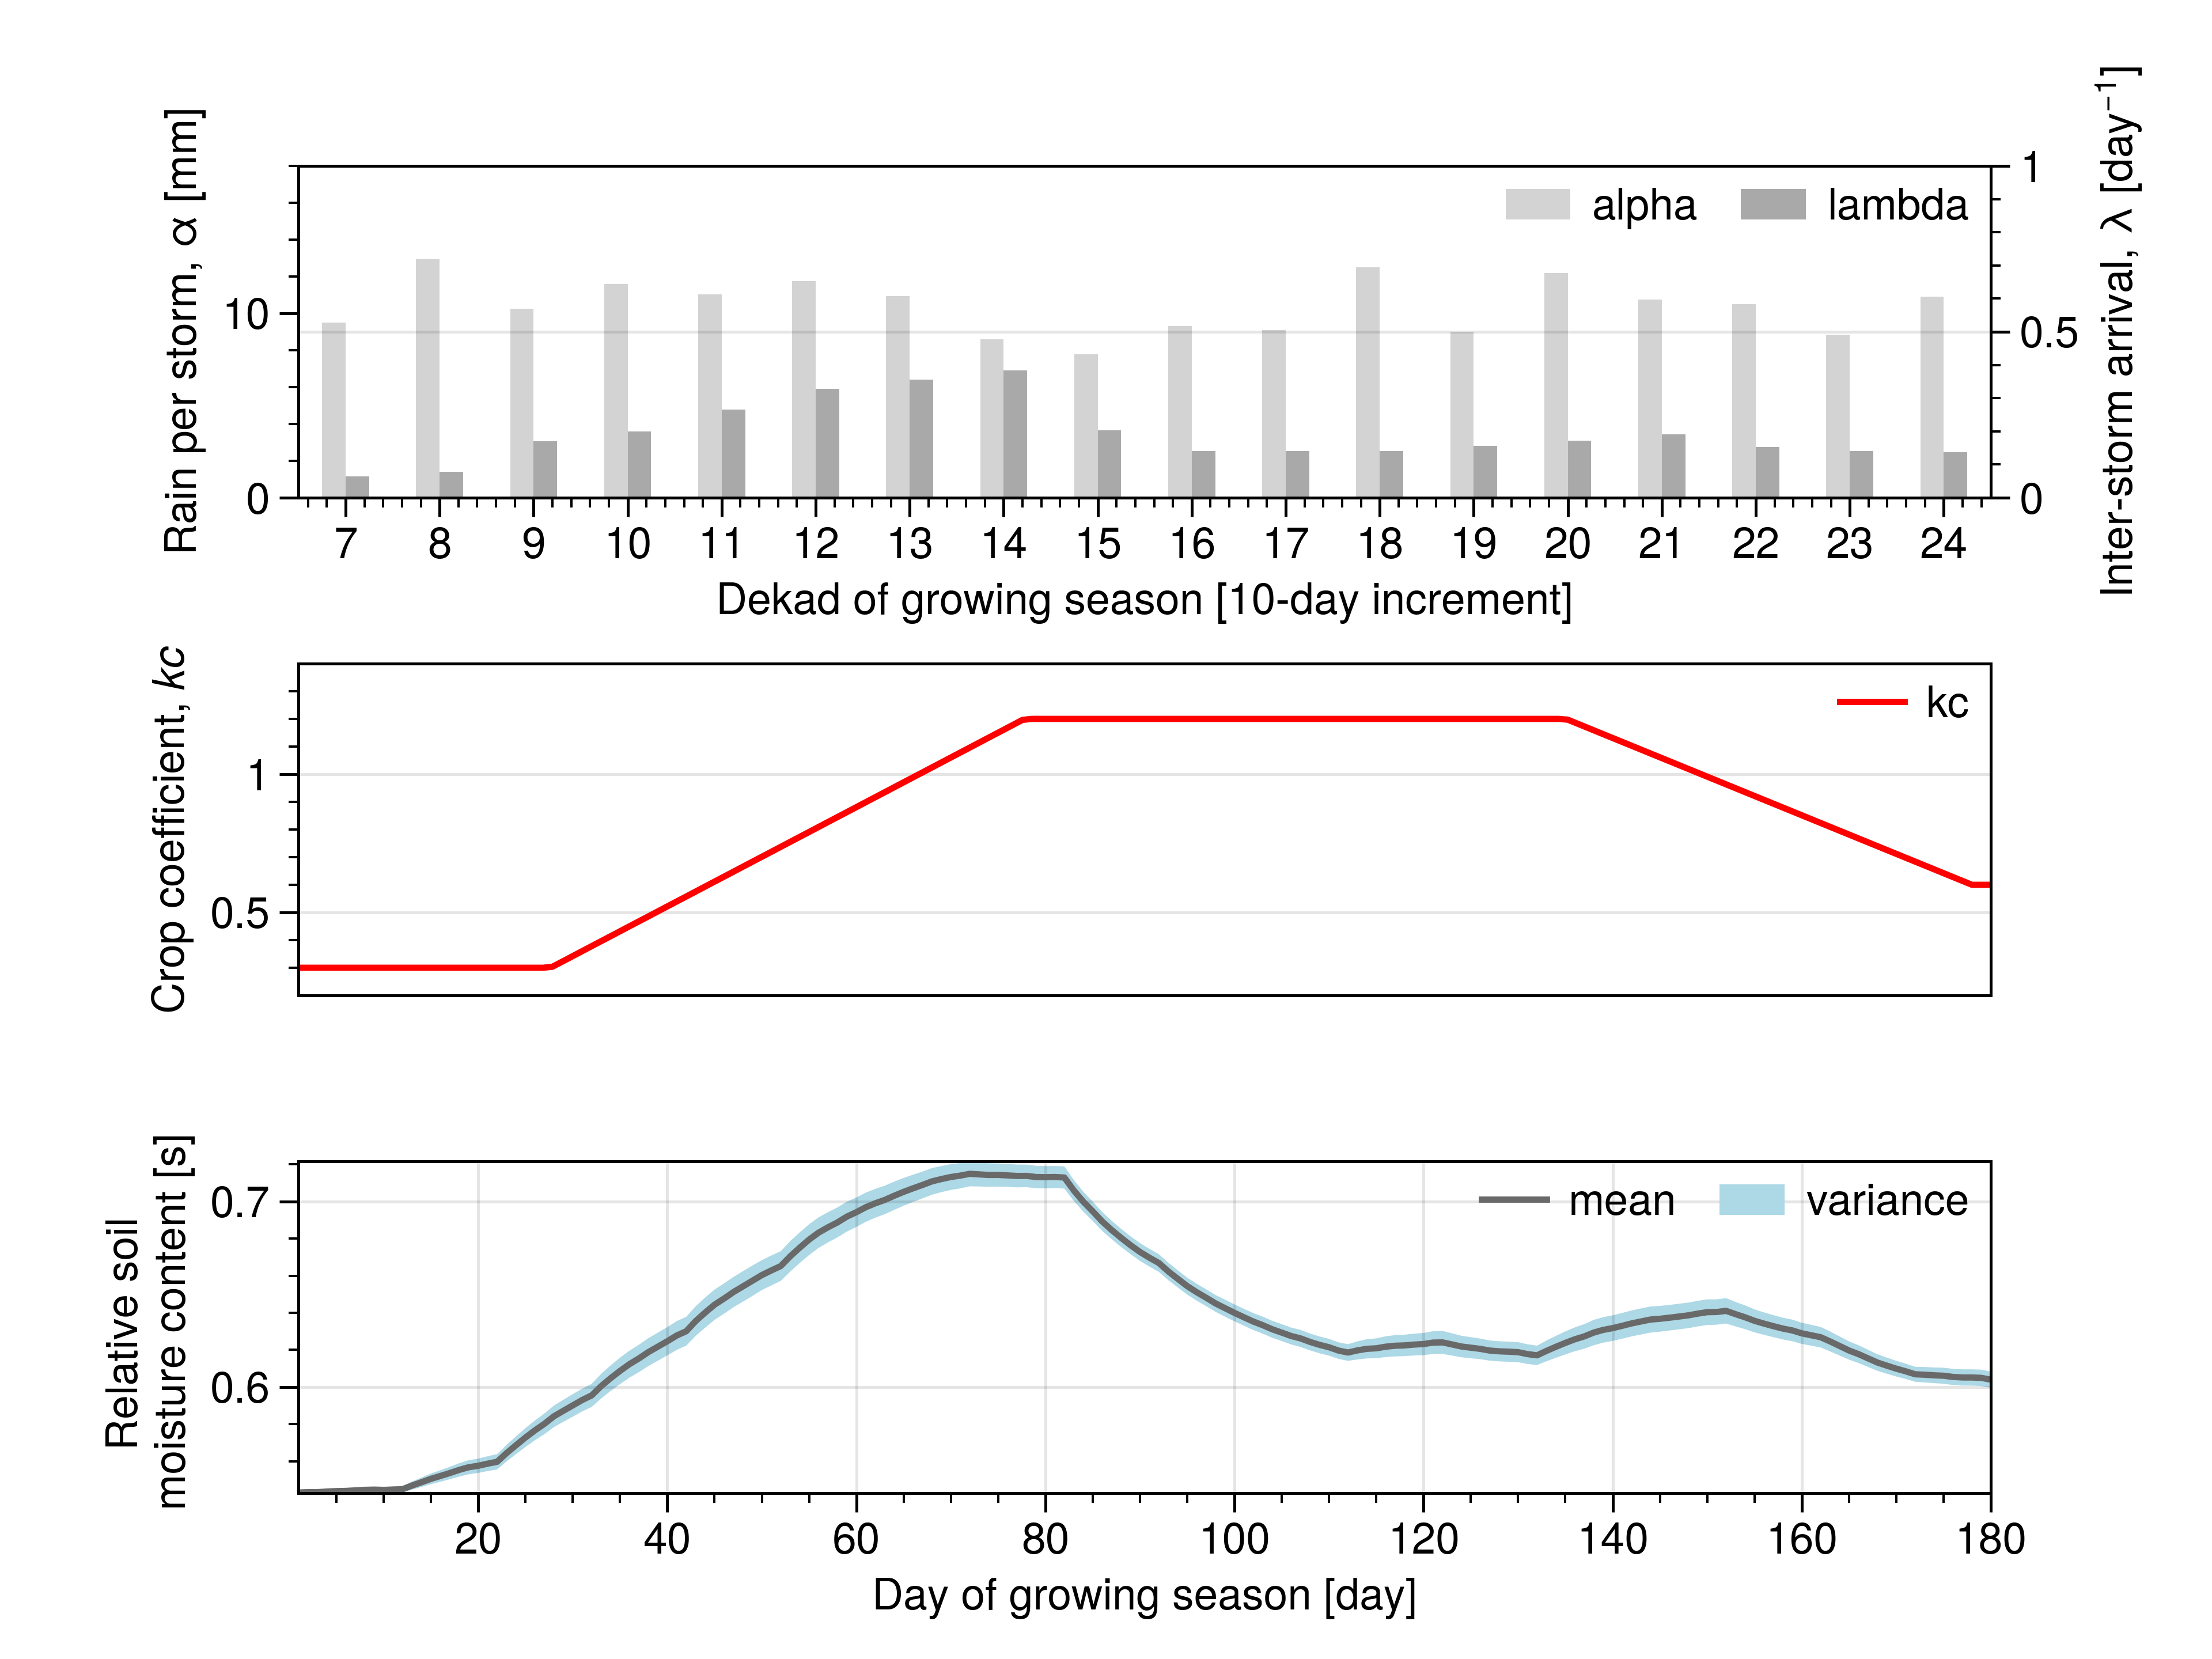
\includegraphics[width=100mm]{fig5_threefigs_dekadal.png}
\caption{Three non-steady state model parameters: Dekadal alpha and lambda values starting with the dekad of planting (dekad 7, March 2-11 in non-leap year) (top); daily crop coefficient (middle); and daily relative soil moisture (bottom).}
\label{fig:threefigs_dekadal}
\end{figure}

\begin{figure}%[ht]
\centering
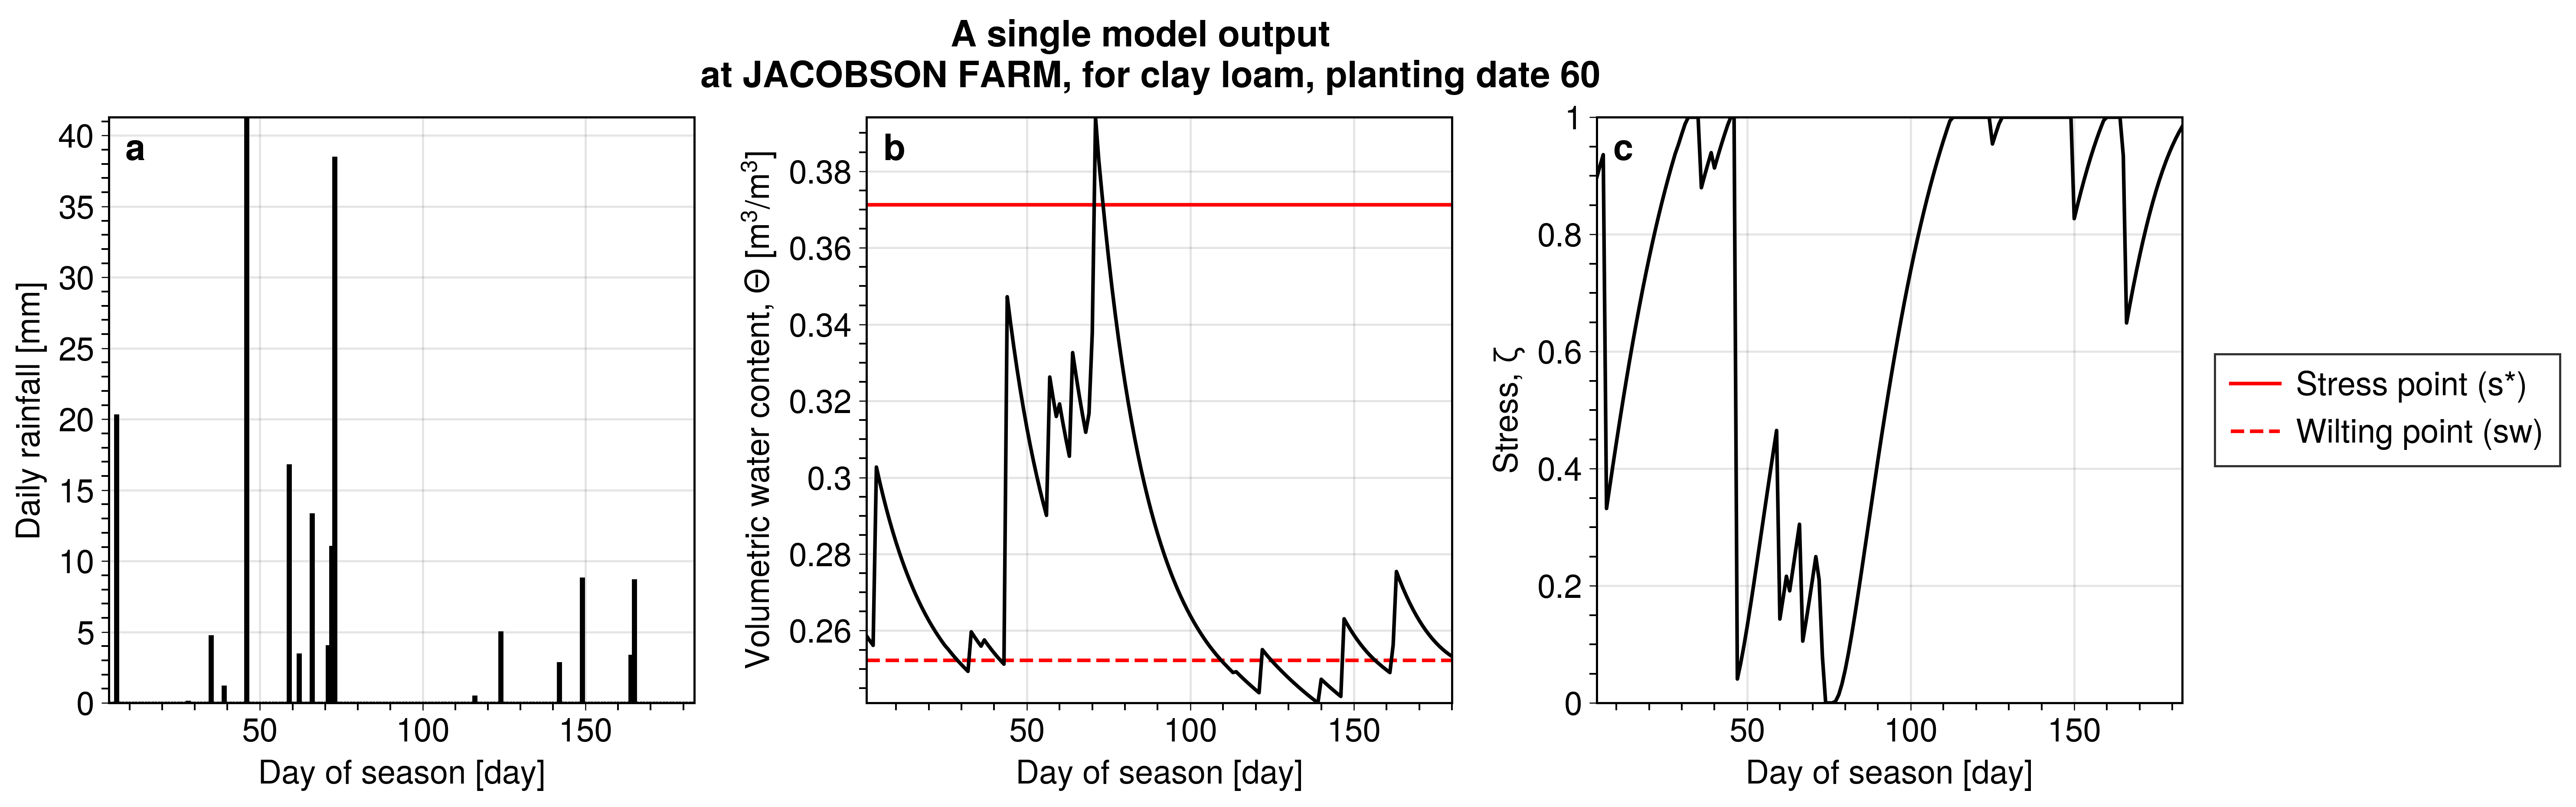
\includegraphics[width=155mm]{fig6_ts.png}
\caption{Time series of precipitation (a), volumetric water content (b), and static stress (c) for a single simulation. Rainfall climatology is determined by Ol Jogi Farm station data, soil texture is clay loam, maize variety is 180 days, and planting date is day of year 60. Soil wilting point is red dashed line. Stress point (the point at which transpiration starts being reduced) is the solid red line. For a clay loam soil the stress point is 0.37128 m3/m3 and the wilting point is 0.25228 m3/m3.
}
\label{fig:fig1}
\end{figure}


\begin{figure}%[ht]
\centering
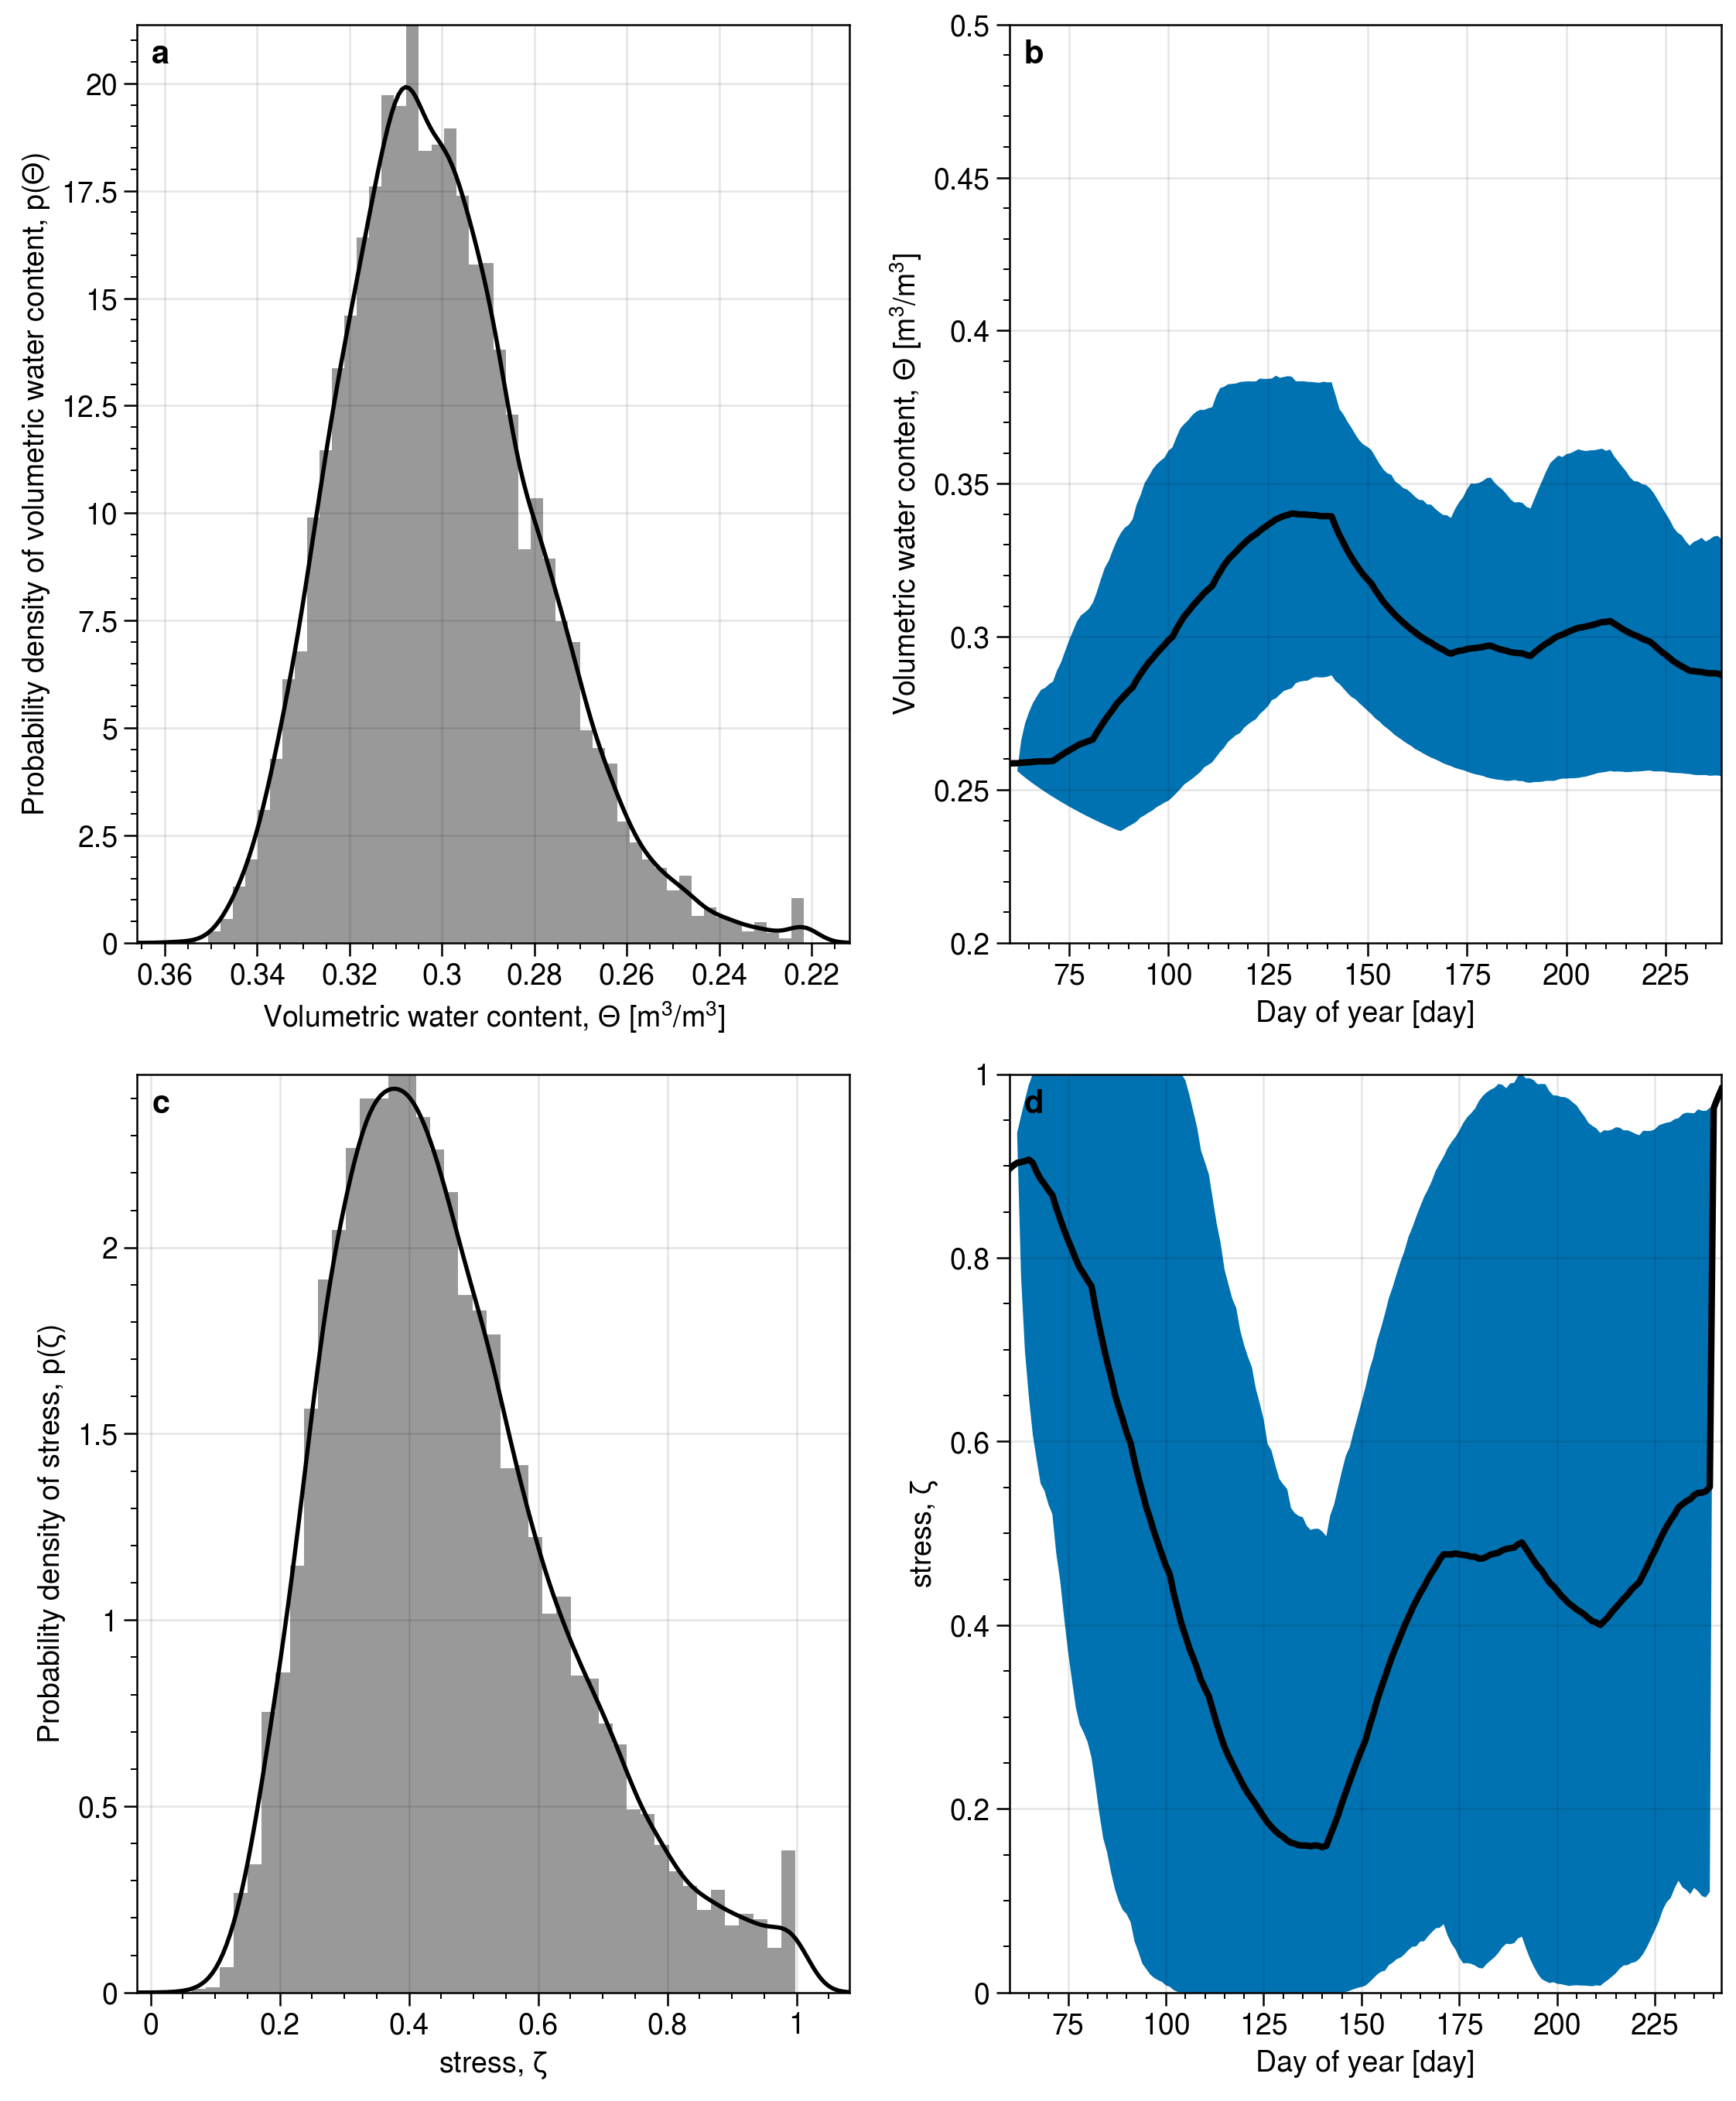
\includegraphics[width=100mm]{fig7_PDFs.png} 
\caption{Probability distribution functions and time series of average soil moisture and stress with 90 and 10\% confidence intervals for 10,000 simulations. Model parameters used are the same as those in Figure \ref{fig:fig1}.}
\label{fig:fig2}
\end{figure}

\begin{figure}%[ht]
\centering
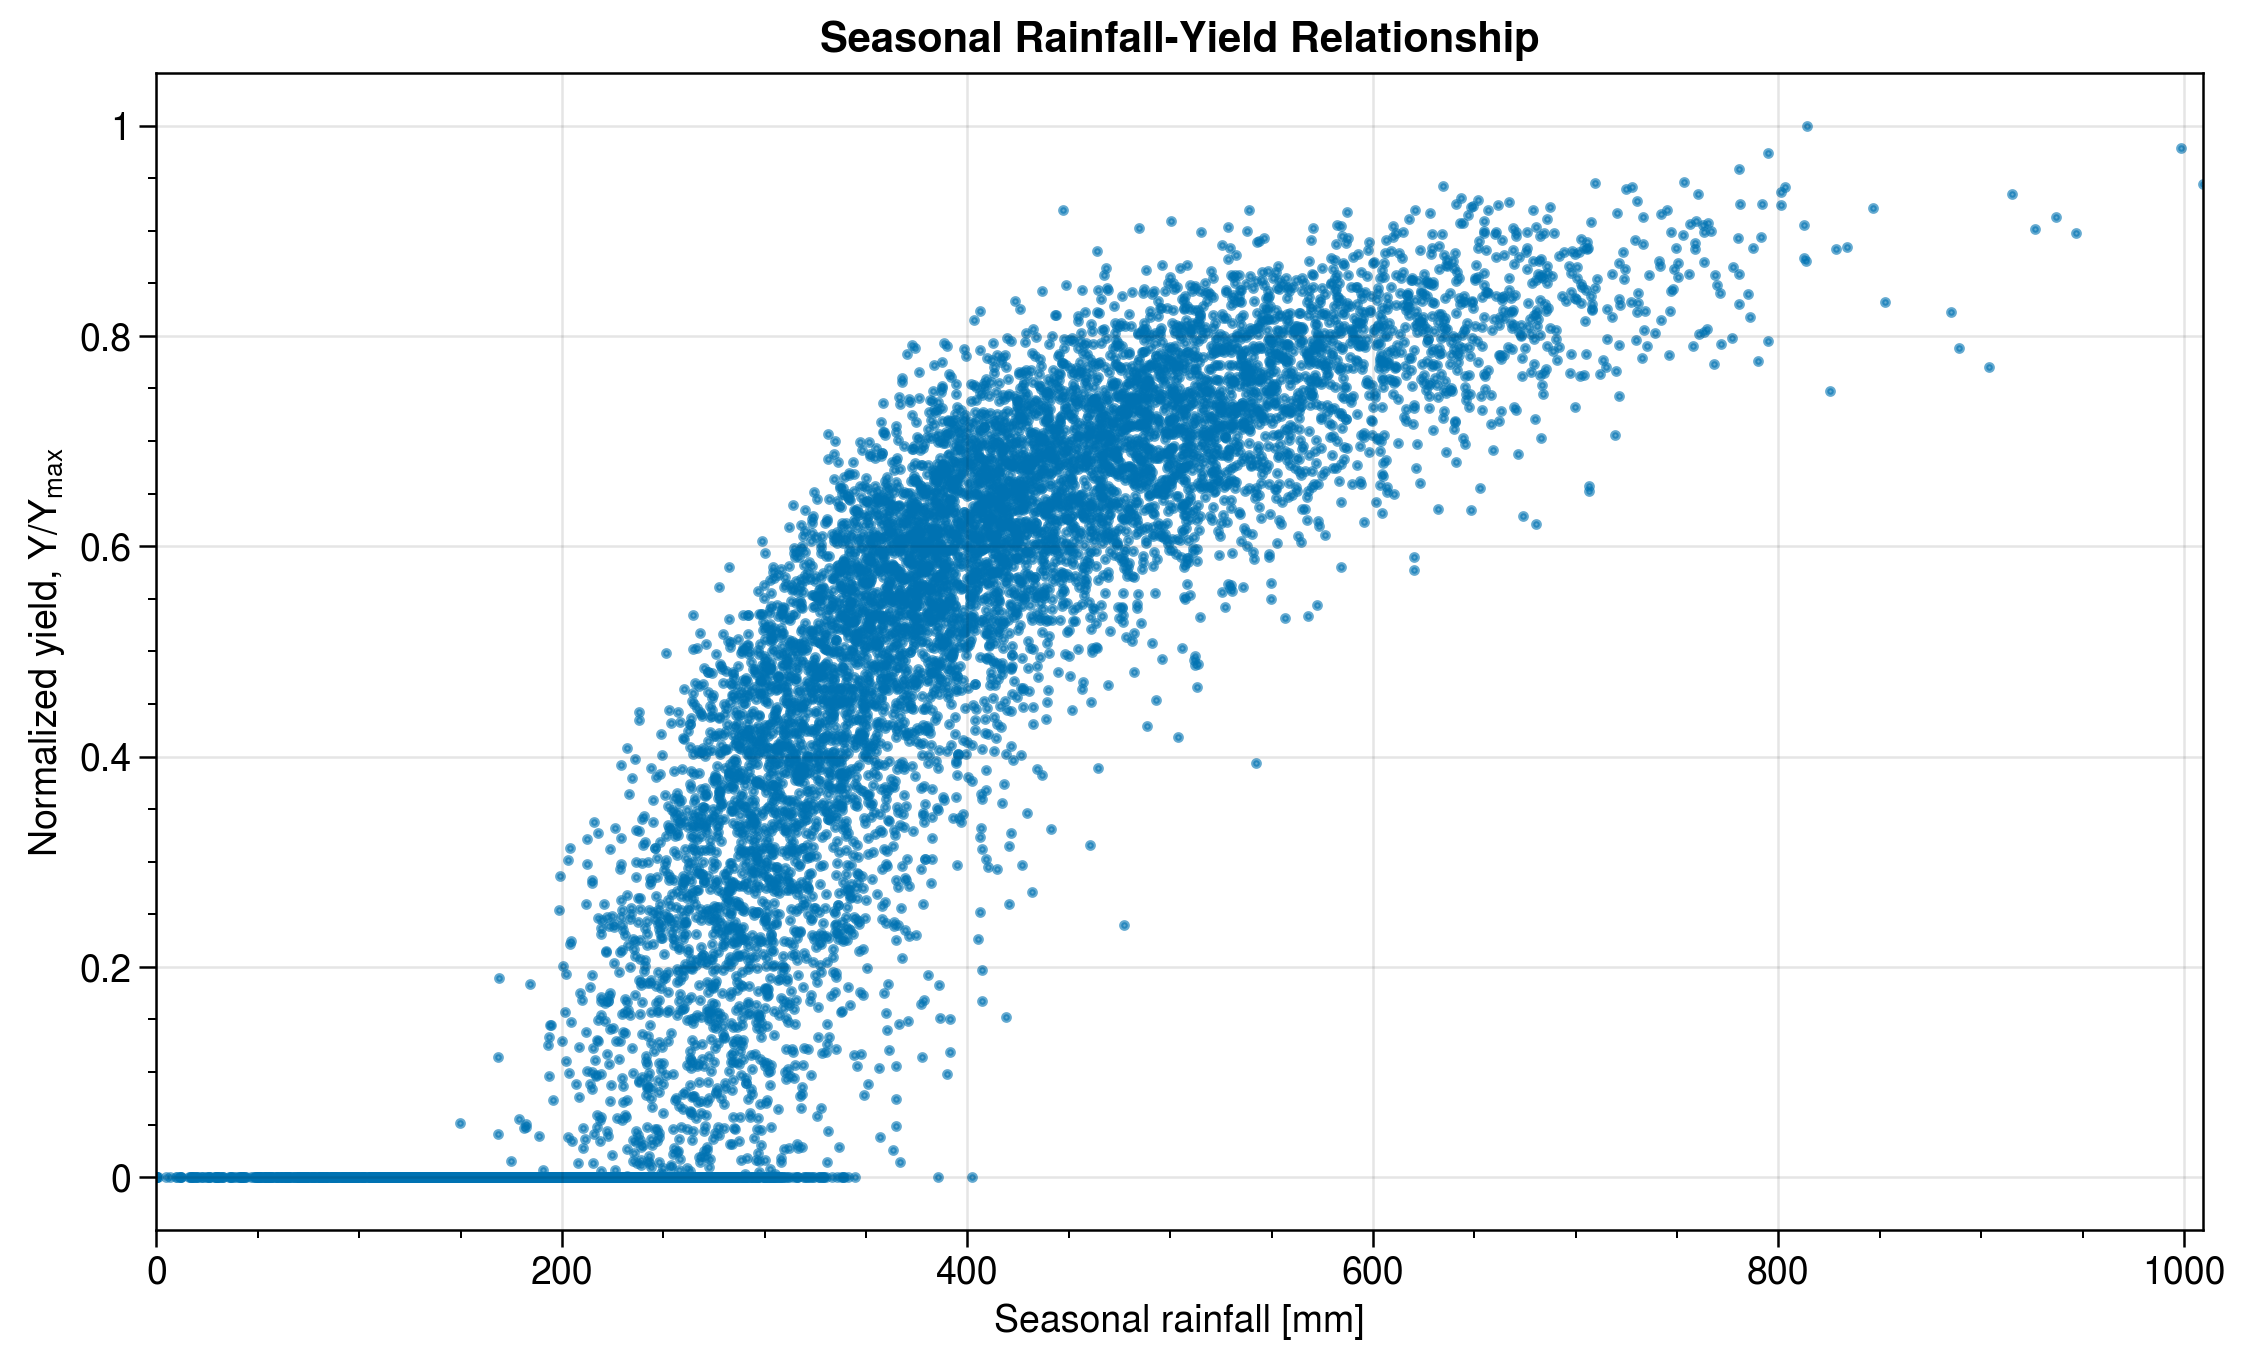
\includegraphics[width=120mm]{fig8_dyn-stress.png}
\caption{Scatterplot of seasonal rainfall and yield for 180-day maize and study site conditions. End of season yields are normalized by the maximum yield, 3.2 t/ha.}
\label{fig:dynstress}
\end{figure}

\begin{figure}%[ht]
\centering
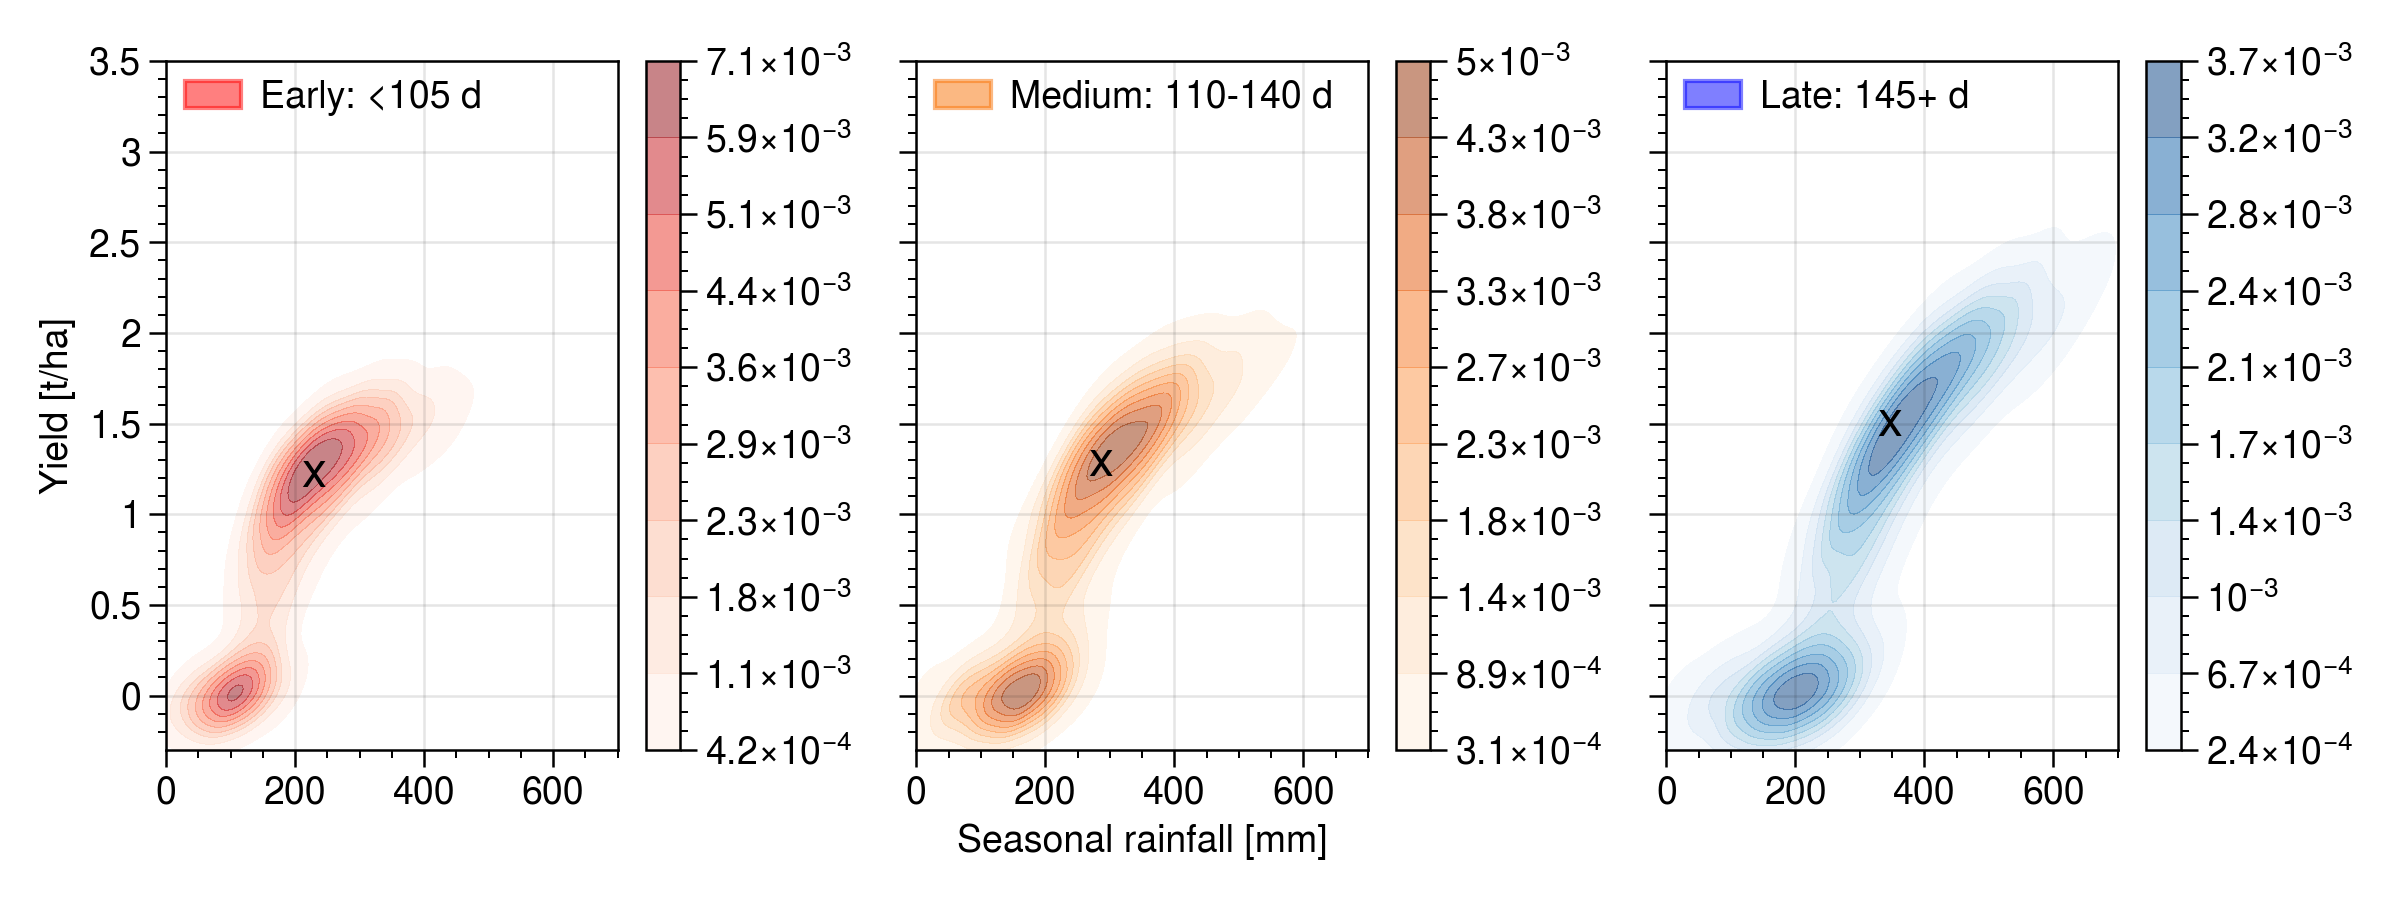
\includegraphics[width=140mm]{fig9_varietiesPDF.png}
\caption{Joint probability distribution of three maize varieties categories. The average rainfall and yield for each subplot is denoted with `x'. Non-zero values of yield were used to calculate this average.}.
\label{fig:varietiesPDF}
\end{figure}

% \begin{figure}%[ht] 
% \centering
% \includegraphics[width=140mm]{varietiesPDF_alt.png}
% \caption{Joint PDF of three maize varieties. Top: Joint probabilities plotted together with color bars showing range of probabilities. Y-axis is yield normalized by maximum yield per variety. Bottom: Three varieties plotted separately. Symbol denotes average rainfall and yield for each variety}.
% \label{fig:varietiesPDF_alt}
% \end{figure}

% \begin{figure}%[ht]
% \centering
% \includegraphics[width=140mm]{cropoutcomes.png}
% \caption{Historical change in crop failure (subplot a) and yield (subplot b) for Jacobson Farm climatology. We defined three eras of rainfall conditions in which we set the alpha and lambda parameters based on the relative trend line in Figure \ref{fig:jacobson}.}
% \label{fig:cropoutcomes}
% \end{figure}

\begin{figure}%[ht]
\centering
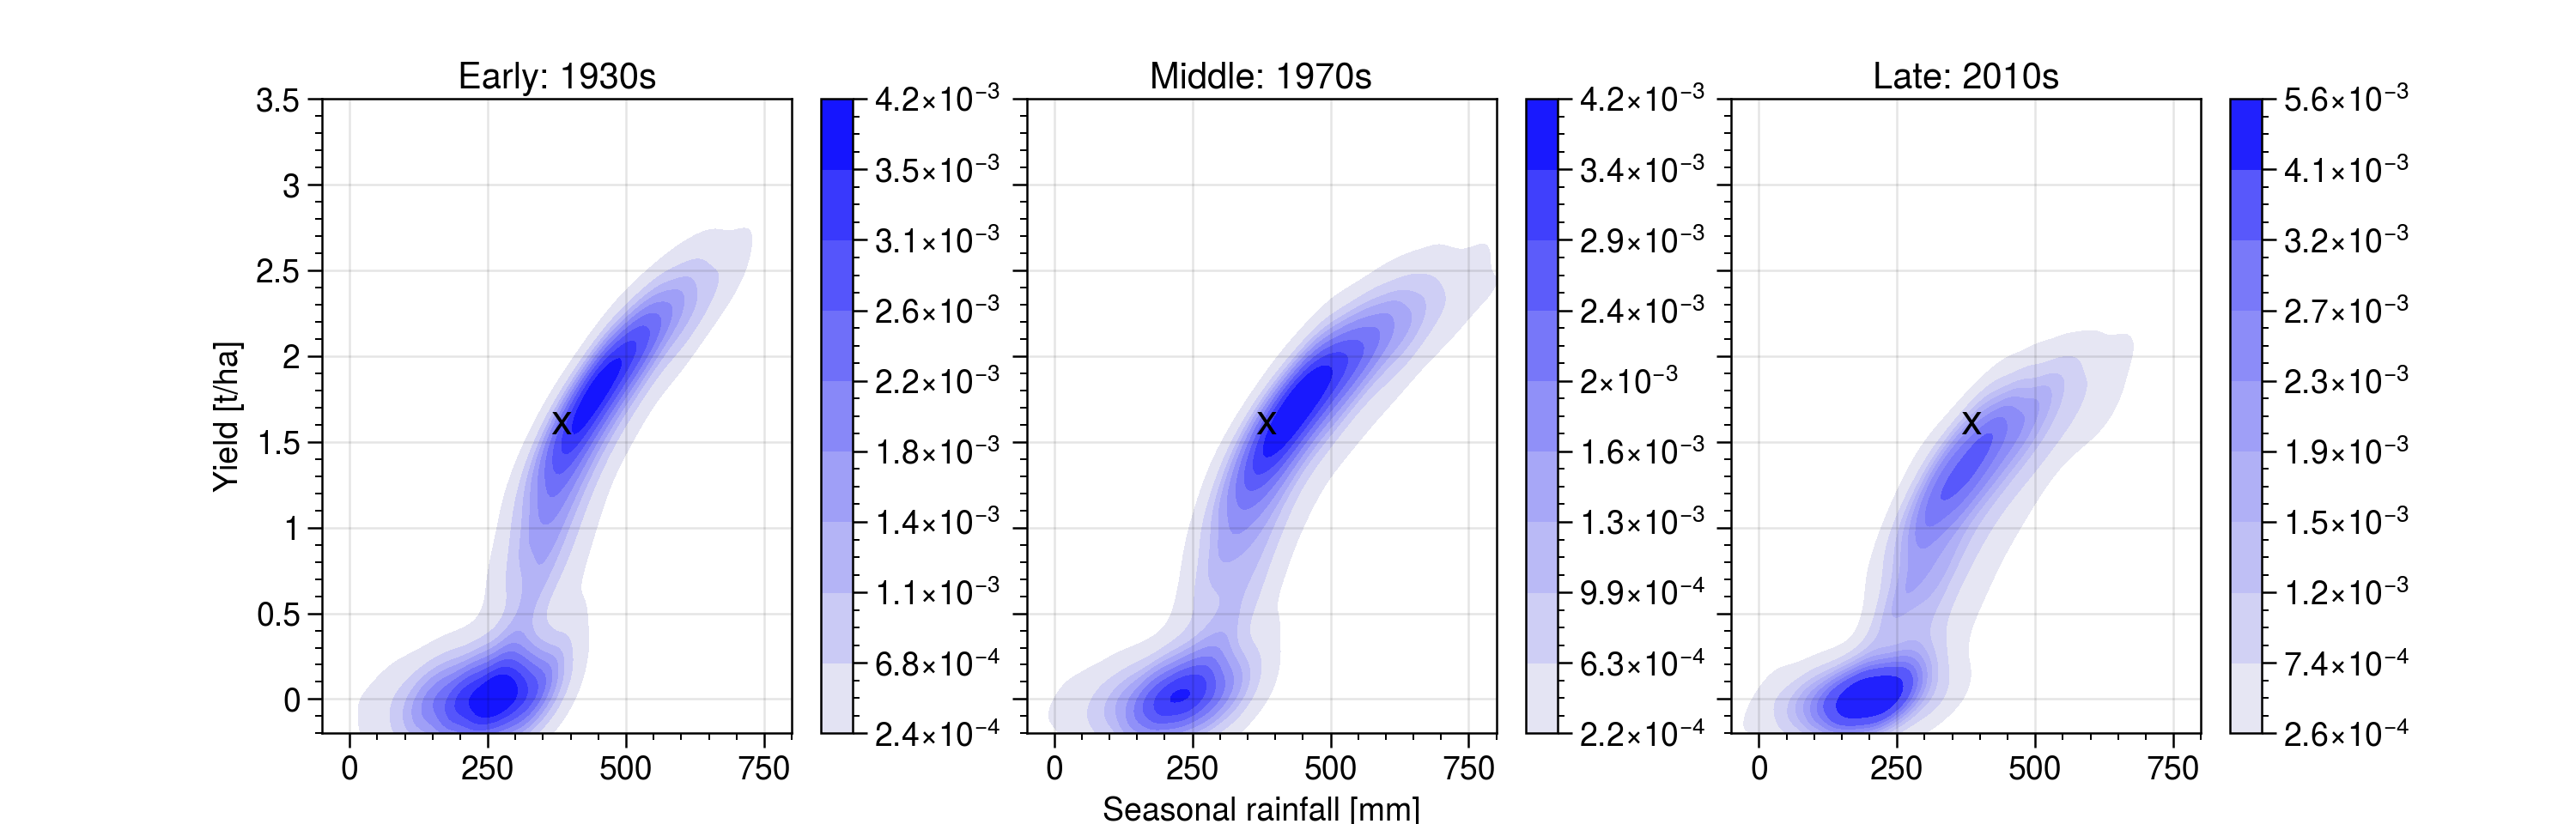
\includegraphics[width=140mm]{fig10_erasPDF.png}
\caption{Historical change in seasonal rainfall and yields for Jacobson Farm climatology. We defined three eras of rainfall conditions in which we set the alpha and lambda parameters based on the relative trend line in Figure \ref{fig:jacobson}. The average rainfall and yield for each subplot is denoted with `x'. Non-zero values of yield were used to calculate this average.}
\label{fig:cropoutcomesPDF}
\end{figure}


\begin{table}
\caption{Summary statistics for three maize variety categories.}
\begin{tabular}{lccc}
\hline
Maize Variety &  Average Rainfall (mm) &  Average Yield (t/ha) &  Crop Failure (\%) \\
\hline
Early ($<$ 105 d) & 212.7 & 1.13 & 18.00 \\
Medium (110 - 140 d) & 255.5 & 1.13 & 25.14 \\
Late (145 + d) & 299.8 & 1.32 & 35.63 \\
\hline
\end{tabular}
\label{varieties}
\end{table}

\begin{table}
\caption{Summary statistics for historical trends in crop failure and yield. Parameters set to Jacobson Farm with a planting date of day 60 and a 180 day maize variety.$^{a}$}
\centering
\begin{tabular}{l ccc}
\hline
 Metric  & Early: 1930s & Avg: 1970s & Late: 2010s  \\
\hline
   Average Seasonal Alpha (mm) & 5.71 & 8.33 & 10.99   \\
   Average Seasonal Lambda (day$^{-1}$) & 0.35 & 0.26 & 0.16  \\
   Average Seasonal Rainfall (mm) & 363.7 & 388.0 & 316.3  \\
   SD Rainfall & 138.5 & 154.6 & 135.1 \\
   CV Rainfall & 0.38 & 0.40 & 0.43 \\
   Average Yield (t/ha) & 0.95 & 1.12 & 0.77 \\
   Probability of Crop Failure (\%) & 38.3 & 26.7 & 34.1 \\
\hline
\multicolumn{2}{l}{$^{a}$SD, standard deviation. CV, coefficient of variation.}
\end{tabular}
\label{summary_cropoutcomes}
\end{table}


\section{Discussion} \label{discussion}

\subsection{Rainfall trends and impacts on maize production}

Warming global temperatures directly cause inter-annual variability in rainfall---i.e., the shift towards fewer and more intense storms \cite{IPCC2007}---as observed at Jacobson Farm and other gauges in the field site (Table \ref{table:mk}). With air temperatures and atmospheric water vapor rising in East Africa as well as globally, extreme precipitation events are expected to increase \cite{trenberth2011changes,christiansen2007}. We find that while rainfall seasonal totals are not changing, the inter-storm arrival rate and average storm depth have changed in several sites in Laikipia, Meru and Nyeri counties.

When considering the extremes of the 80-year rainfall record (i.e. 1930s versus 2010s rainfall climatology), we see changes in cropping outcomes among maize farmers. Overall, we find a downward trend in yield and an upward trend in crop failure due to the pattern of decreased rainfall frequency and increased rainfall intensity. Because the inter-storm arrival rate has decreased by half and the average storm size has roughly doubled it is becoming more difficult to grow maize in these rainfed systems. Previous work has demonstrated the similar finding that the intensity and duration of individual rainfall events is more important for hydrological partitioning of precipitation than annual or seasonal totals \cite{taylor2013evidence,apurv2017understanding,singer2017deciphering,adloff-inreview}. Additionally, we see an increase in the coefficient of variation in rainfall showing that farmers experience increasingly variable rainfall conditions.

Previous studies have sparked concern over the future of rainfall in East Africa and formed a consensus about the role of climate change in influencing rainfall patterns \cite{nicholson2017climate, shongwe2011projected, adloff-inreview}. Specifically, these studies have demonstrated negative trends in the magnitude of the long rains (March-May) in East Africa and the Horn of Africa Drylands (HAD) \cite{lyon2012recent,liebmann2014understanding,williams2011westward, funk2018examining,funk2019recognizing}. Other studies have shown regional trends towards more extreme rainfall events \cite{harrison2019identifying}, particularly for the short rains (October-December) \cite{shongwe2011projected,adloff-inreview} and in central Kenya \cite{schmocker2016trends}. Adloff et al. (2020, in review) showed that the HAD received 62\% more extreme rainfall (rainfall events over the 99th percentile) for the short rains between 2003 and 2014 and 58\% more extreme rainfall in the long rains between 1981 and 2001. This further suggests that rainfall in the region is arriving in larger quantities. As we show, this trend will likely contribute to decreased end of season yields and increased rates of crop failure due to the timing and nature of rainfall and crop water requirements of maize over the season. Increasingly heavy rainfall events pose a threat to crop production due to extreme surface runoff and subsequent erosion or from flood events  \cite{liniger1998grass, liniger1998mountains}. 

We show that maize is becoming increasing difficult to grow under current climatic conditions. Small-scale producers depend on reliable rainfall. They must avoid both extreme storms (i.e. no flooding) and dry spells in order to attain end of season yields that are profitable. Our results show that despite having seasonal rainfall totals that should be adequate for maize growth, the end of season yields and chance of crop failure are highly variable. This is because the crop coefficient of maize does not align with the periods of highest rainfall when planting is conducted in early March and in these systems where irrigation may be absent. For this reason, hybrid maize has been developed to withstand variable rainfall and drought during the growing season.

%Second section
\subsection{Cultivar choice moderates exposure to stress}

We investigate the effect of cultivar choice on crop failure and yield by simulating the growth of maize varieties with early, medium and late maturation periods, which each experience differing levels of water stress over the growing season. We show that modest decreases in relative water content lead to dramatic increases in the water stress of simulated maize. When the length of the growing period is shortened for an early-maturing crop to reach the flowering and grain-filling phenological stages faster, there is a reduced chance of exposure to water deficits. Our simulated daily rainfall is governed by parameters set in dekadal (10-day) increments in which rainfall is more likely during the long rains (approx. dekads 11-14) and the short rains seasons (approx. dekads 25-34). A long-maturing 180-day variety which is planted on March 1 would be harvested at the end of August, which is just shy of the onset of the short rains. In contrast, an early-maturing variety would grow for a shortened duration and would reach critical stages of its development during the peak of the long rains season. For the 180-day variety simulations, we see the highest crop coefficient between approximately days 80 and 140; however, during this period there is a large decrease in the inter-storm arrival rate due to the cessation of the long rains. Although this period is critical for maize development as the crop has flowered and begins to grain-fill, the soil moisture content declines because of the lack of rain and the high water requirements. Because of rainfall non-stationarity within seasons, crops experience differing stress environments based on when and how long they grow. 

Cultivar choice is one of the primary adaptation strategies that farmers can control to minimize the stress experienced by the crop. We show that early-maturing crops are the best choice under lower levels of rainfall and have the lowest probability of crop failure. Late-maturing crops will produce higher yields in the simulations that do not fail, however, they have a higher risk of crop failure. Thus, early-maturing varieties are the least likely to fail just on the basis of requiring less time to grow. Furthermore, early-maturing varieties are often bred or have been genetically modified to be drought tolerant. Drought tolerance is often developed for a specific set of environmental conditions and thus can be hyper-localized. For low levels of rainfall there is a larger spread in yield outcomes for all varieties due to the pattern of rainfall within the season. As previously discussed, the intensity and timing of rainfall more than seasonal totals matters for determining outcome.

In a survey of 500 East African farming households, \citeA{erenstein2011characterization} found that the most desired attribute of maize varieties was yield potential followed by early maturity. These characteristics were perceived to be more important than drought tolerance. Maize cultivars can exhibit one of two traits: drought avoidance as in the case of early-maturing varieties and drought tolerance in the case of hybrids that are bred to tolerate reduced available water. Early-maturing varieties are considered drought avoidant because they are thought to complete their most drought-sensitive stage (flowering) before a drought occurs such as at the ending of a growing season \cite{barron2003dry, morris2001assessing}.

We show that by growing a late-maturing variety, the crop is still subject to terminal drought and crop failure due to the timing of rainfall throughout the season. However, a trade-off exists in selecting a late-maturing variety. As shown in the empirical data of maize cultivars and yield (Figure \ref{fig:ksc}), there is an opportunity for higher yields for late-maturing maize varieties. In cases where farmers who do not have access to irrigation and would prefer a crop that has a greater chance of success despite a potential yield penalty, they may prefer early-maturing crops \cite{barron2003dry}.

There are two possibilities that plant breeders and farmers can elect for: to optimize for survival by minimizing the variance of stress experienced by the crop or to optimize for greater biomass in order to get the maximum yield. In light of this, farmers may be interested in maximizing their yield as well as limiting crop failure by planting a medium-maturing variety. However, in areas with high rainfall variability there might be reason to plant only early-maturing varieties either with the intent of minimizing crop failure or in order to double crop within the season. In these settings where a farmer’s goal is to prevent crop failure, early- and extra early-maturing varieties are more effective for a planting date of the first dekad of March 1 as described in our model.  There may be a role for varieties with other maturity durations when using different planting dates. 

\subsection{Declining yields, increasing crop failure rates and household-level impacts}
% Yield and crop failure rates in the context of climatological trends

The increased variability in rainfall has serious implications for agriculture in East Africa and other regions of the African continent where large portions of the population suffer from food insecurity \cite{funk2009declining}. Even if the mean annual rainfall does not change significantly, changes to the pattern of rainfall within the season may make it difficult for farmers to practice agriculture as they have done so in the past. As shown in the temporal analysis of rainfall trends, the timing and distribution of rainfall has changed within one to two generations.

Climate change and climate variability impacts can shock the economic system by altering food prices and so affecting food demand, nutrition, and human livelihoods \cite{herrero2010climate}. We have already shown that season-to-season variability in rainfall is high, and the distribution of rainfall in addition to the total is of paramount importance to Kenyan agriculture. In Kenya, declines in per capita maize production have been reported for certain regions \cite{funka2018a}. Much of this change is due to variable seasonal rainfall and the incidence of crop failure.  Our results are consistent with work that projects reduced rainfed maize yields in Kenya \cite{herrero2010climate, thornton2010adapting}. While yield gains have been projected for certain highland areas in the temperate areas of Kenya \cite{thornton2010adapting}, farmers in the semiarid and arid lowlands are predicted to experience diminished yields, likely forcing them to sow varieties with shorter maturity periods. 

In order to capitalize on any potential yield increases in the highlands and reduce as much as possible the decreased yields in the majority of Kenya, further investment in new varieties, improved inputs, and services will be needed \cite{herrero2010climate, Hansen2011-bk}. Access to irrigation and water harvesting more generally will be an important way for farmers to buffer negative climate impacts. In this region in central Kenya, access to irrigation resources is not ubiquitous and even those farmers with access to irrigation experience high spatial and temporal variability in its availability \cite{gower2016modeling}. \citeA{mccord2018assessing} show that farmers in the Mount Kenya region with greater relative variability in water flow from irrigation are more likely to uptake adaptation measures such as choosing new seed varieties. This is a positive indication that perhaps the agriculturalists who are more impacted by rainfall variability due to reduced irrigation access are likely to employ adaptation measures or at least experiment with those measures such as changing to an early- or extra-early maturing varieties \cite{mccord2018assessing}. 

\subsection{Study Limitations and Future Research}
We made some important assumptions in our model, a common practice in such studies \cite <e.g.>[]{challinor2009crops, tesfaye2016targeting}. First, other than the rainfall climatology and the crop coefficient all other variables were constant. We do not simulate the effect of inputs such as fertilizer application or irrigation use. The model assumes that nutrients like nitrogen are available in adequate quantities that do not limit growth crop and yield. Second, we do not simulate other crops which might be intercropped with maize (e.g. beans, potatoes), and we do not simulate crop rotation. Additional studies may begin with any of these assumptions to further evaluate their effects on maize production.

Future studies would benefit from adding empirical agronomic or decision-making data as inputs or validation datasets. Our study has shown that available water content is lowest during the latter part of the season when the crop coefficient is the highest and the rainfall slackens. A follow-up study could investigate the intra-seasonal nature of water stress to demonstrate what duration of stress during the season makes the largest impact in terms of yield. To answer this question, an empirical dataset is needed that includes both intra-seasonal stress dynamics and end of season yields. Additionally, we did not constrain the behavior of early-, medium-, and late-maturing varieties other than changing the length of their growing periods. Early-maturing maize is often bred or genetically modified to be drought tolerant and thus should reduce the probability of crop failure. These constraints could be added as parameters in the dynamic water stress calculation or by altering the crop coefficient for hybrid maturities. Field-collected data or on-farm trials would be needed to constrain these parameters.

\section{Conclusions} \label{conclusion}

This stochastic ecohydrological model represents conditions that will become more common as climate variability and climate change alters rainfall in tropical and semiarid systems. By using historical rainfall to generate stochastic conditions for average depth and probability of rainfall we simulated a dryland environment for small-scale producers. We considered a common crop choice (maize), soil type, and planting decisions (i.e. timing of planting) that represents hundreds of millions of small-scale producers in regions vulnerable to climate change and variability. We investigated the role of rainfall variability in explaining current and past agricultural outcomes such as yield and likelihood of total crop failure. Additionally, we show the importance of cultivar choice in determining yield potentials and the vulnerability of late-maturing varieties to rainfall variability. 

How we characterized rainfall variability and its relationship to crop phenology (crop coefficient) was a novel contribution to a field where hydrologic processes are often considered separate from the phenology of the crop. We defined water availability as a function of stochastic rainfall and soil parameters whereas the crop coefficient governed water demand. Our model especially considers the rainfall depth and frequency (alpha and lambda) parameters as forces that drive stochastic rainfall. Thus we can simulate non-steady state soil moisture which changes over the course of the season due to shifts in the water required by the crop.

In the face of climate change, where direct changes in water availability, temperature, and increased prevalence of pest and diseases are possible, farmers can adapt through two key management strategies: choice of cultivar maturities and planting dates \cite{van2013yield}. Farmers need to select locally relevant planting dates and cultivars with appropriate maturities to minimize crop failure. Future study on the role of planting dates would illuminate the relative advantages of early- to late-maturing crops planted during Kenya's two primary rainy seasons. With appropriate climate data and locally-relevant agronomic conditions, this type of modeling can be used as a heuristic to improve our understanding of the impacts of climate variability on farming outcomes in other contexts. 


%%

%  Numbered lines in equations:
%  To add line numbers to lines in equations,
%  \begin{linenomath*}
%  \begin{equation}
%  \end{equation}
%  \end{linenomath*}



%% Enter Figures and Tables near as possible to where they are first mentioned:
%
% DO NOT USE \psfrag or \subfigure commands.
%
% Figure captions go below the figure.
% Table titles go above tables;  other caption information
%  should be placed in last line of the table, using
% \multicolumn2l{$^a$ This is a table note.}
%
%----------------
% EXAMPLE FIGURES
%
% \begin{figure}
% \includegraphics{example.png}
% \caption{caption}
% \end{figure}
%
% Giving latex a width will help it to scale the figure properly. A simple trick is to use \textwidth. Try this if large figures run off the side of the page.
% \begin{figure}
% \noindent\includegraphics[width=\textwidth]{anothersample.png}
%\caption{caption}
%\label{pngfiguresample}
%\end{figure}
%
%
% If you get an error about an unknown bounding box, try specifying the width and height of the figure with the natwidth and natheight options. This is common when trying to add a PDF figure without pdflatex.
% \begin{figure}
% \noindent\includegraphics[natwidth=800px,natheight=600px]{samplefigure.pdf}
%\caption{caption}
%\label{pdffiguresample}
%\end{figure}
%
%
% PDFLatex does not seem to be able to process EPS figures. You may want to try the epstopdf package.
%

%
% ---------------
% EXAMPLE TABLE
%
% \begin{table}
% \caption{Time of the Transition Between Phase 1 and Phase 2$^{a}$}
% \centering
% \begin{tabular}{l c}
% \hline
%  Run  & Time (min)  \\
% \hline
%   $l1$  & 260   \\
%   $l2$  & 300   \\
%   $l3$  & 340   \\
%   $h1$  & 270   \\
%   $h2$  & 250   \\
%   $h3$  & 380   \\
%   $r1$  & 370   \\
%   $r2$  & 390   \\
% \hline
% \multicolumn{2}{l}{$^{a}$Footnote text here.}
% \end{tabular}
% \end{table}

%% SIDEWAYS FIGURE and TABLE
% AGU prefers the use of {sidewaystable} over {landscapetable} as it causes fewer problems.
%
% \begin{sidewaysfigure}
% \includegraphics[width=20pc]{figsamp}
% \caption{caption here}
% \label{newfig}
% \end{sidewaysfigure}
%
%  \begin{sidewaystable}
%  \caption{Caption here}
% \label{tab:signif_gap_clos}
%  \begin{tabular}{ccc}
% one&two&three\\
% four&five&six
%  \end{tabular}
%  \end{sidewaystable}

%% If using numbered lines, please surround equations with \begin{linenomath*}...\end{linenomath*}
%\begin{linenomath*}
%\begin{equation}
%y|{f} \sim g(m, \sigma),
%\end{equation}
%\end{linenomath*}

%%% End of body of article

%%%%%%%%%%%%%%%%%%%%%%%%%%%%%%%%
%% Optional Appendix goes here
%
% The \appendix command resets counters and redefines section heads
%
% After typing \appendix
%
%\section{Here Is Appendix Title}
% will show
% A: Here Is Appendix Title
%
%\appendix
%\section{Here is a sample appendix}

%%%%%%%%%%%%%%%%%%%%%%%%%%%%%%%%%%%%%%%%%%%%%%%%%%%%%%%%%%%%%%%%
%
% Optional Glossary, Notation or Acronym section goes here:
%
%%%%%%%%%%%%%%
% Glossary is only allowed in Reviews of Geophysics
%  \begin{glossary}
%  \term{Term}
%   Term Definition here
%  \term{Term}
%   Term Definition here
%  \term{Term}
%   Term Definition here
%  \end{glossary}

%
%%%%%%%%%%%%%%
% Acronyms
%   \begin{acronyms}
%   \acro{Acronym}
%   Definition here
%   \acro{EMOS}
%   Ensemble model output statistics
%   \acro{ECMWF}
%   Centre for Medium-Range Weather Forecasts
%   \end{acronyms}

%
%%%%%%%%%%%%%%
% Notation
%   \begin{notation}
%   \notation{$a+b$} Notation Definition here
%   \notation{$e=mc^2$}
%   Equation in German-born physicist Albert Einstein's theory of special
%  relativity that showed that the increased relativistic mass ($m$) of a
%  body comes from the energy of motion of the body—that is, its kinetic
%  energy ($E$)—divided by the speed of light squared ($c^2$).
%   \end{notation}




%%%%%%%%%%%%%%%%%%%%%%%%%%%%%%%%%%%%%%%%%%%%%%%%%%%%%%%%%%%%%%%%
%
%  ACKNOWLEDGMENTS
%
% The acknowledgments must list:
%
% >>>>	A statement that indicates to the reader where the data
% 	supporting the conclusions can be obtained (for example, in the
% 	references, tables, supporting information, and other databases).
%
% 	All funding sources related to this work from all authors
%
% 	Any real or perceived financial conflicts of interests for any
%	author
%
% 	Other affiliations for any author that may be perceived as
% 	having a conflict of interest with respect to the results of this
% 	paper.
%
%
% It is also the appropriate place to thank colleagues and other contributors.
% AGU does not normally allow dedications.


\acknowledgments
%Enter acknowledgments, including your data availability statement, here.
The model output data that support the findings of the study are available on the Github repository [enter link here (link will be added upon acceptance)]. Noah Spahn provided consultations to improve computational efficiency in the model. %The data that support the findings from the historical rainfall trends are available upon reasonable request from the corresponding author. 
CETRAD in Nanyuki, Kenya provided us with the historical rain gauge dataset.   
The research was supported by the National Science Foundation WSC-Category 2  grant awarded to KKC (Award No. 1801251 and 1360421). 

%% ------------------------------------------------------------------------ %%
%% References and Citations

%%%%%%%%%%%%%%%%%%%%%%%%%%%%%%%%%%%%%%%%%%%%%%%
%
% \bibliography{<name of your .bib file>} don't specify the file extension
%
% don't specify bibliographystyle
%%%%%%%%%%%%%%%%%%%%%%%%%%%%%%%%%%%%%%%%%%%%%%%

\bibliography{mybib}



%Reference citation instructions and examples:
%
% Please use ONLY \cite and \citeA for reference citations.
% \cite for parenthetical references
% ...as shown in recent studies (Simpson et al., 2019)
% \citeA for in-text citations
% ...Simpson et al. (2019) have shown...
%
%
%...as shown by \citeA{jskilby}.
%...as shown by \citeA{lewin76}, \citeA{carson86}, \citeA{bartoldy02}, and \citeA{rinaldi03}.
%...has been shown \cite{jskilbye}.
%...has been shown \cite{lewin76,carson86,bartoldy02,rinaldi03}.
%... \cite <i.e.>[]{lewin76,carson86,bartoldy02,rinaldi03}.
%...has been shown by \cite <e.g.,>[and others]{lewin76}.
%
% apacite uses < > for prenotes and [ ] for postnotes
% DO NOT use other cite commands (e.g., \citet, \citep, \citeyear, \nocite, \citealp, etc.).
%



\end{document}

